\documentclass[10pt]{beamer}
%================================================
%---------------包配置
%================================================
\usepackage{appendixnumberbeamer}
\usepackage{booktabs}
\usepackage[scale=2]{ccicons}
\usepackage{pgfplots}
\usepackage{xspace}
\newcommand{\themename}{\textbf{\textsc{metropolis}}\xspace}
\renewcommand{\raggedright}{\leftskip=0pt \rightskip=0pt plus 0cm}

% 中文支持 - 简化配置
\usepackage[UTF8,scheme=plain]{ctex}

\usepackage{graphicx}
\usepackage{pdflscape}
\usepackage{pdfpages}
\usepackage{verbatim}
\tolerance=1000

% 代码高亮设置
\usepackage{listings}
\lstset{
    basicstyle=\ttfamily\small,
    breaklines=true,
    frame=single,
    backgroundcolor=\color{gray!10}
}

\usepackage{xcolor}
\usepackage[all]{xy}
\usepackage{times}
\usepackage{tikz}
\usepackage{ragged2e}
\usepackage{caption}
\usepackage{subcaption}
\usepackage{float}

\usepackage{indentfirst}
\usepackage{graphicx}

\usepackage{multirow}
\usepackage{multicol}
\usepackage{lipsum}
\usepackage{ragged2e}
\newcommand{\jus}{\justifying}
\apptocmd{\frame}{}{\justifying}{}
\apptocmd{\block}{}{\justifying}{}
\apptocmd{\column}{}{\justifying}{}
\usepackage{enumerate}

\usepackage{etoolbox}
\usepackage{letltxmacro}

\hypersetup{colorlinks,citecolor=verde,linkcolor=orange,urlcolor=verde}
% 使用标准的natbib代替abntex2cite以确保ShareLaTeX兼容性
\usepackage{natbib}
\bibliographystyle{plainnat}

%=============================
\usetheme[sectionpage=none, subsectionpage=progressbar]{metropolis}
\usepgfplotslibrary{dateplot}
\useoutertheme[subsection=false,footline=authortitle]{miniframes}
\setbeamertemplate{footline}[frame number]
\hypersetup{pdfpagemode=FullScreen}
\hypersetup{pdfpagelayout=SinglePage}

\providecommand{\sin}{} \renewcommand{\sin}{\hspace{2pt}\textrm{sen}}
\providecommand{\tan}{} \renewcommand{\tan}{\hspace{2pt}\textrm{tg}}
\setbeamerfont{section in toc}{size=\small}
\setbeamerfont{subsection in toc}{size=\scriptsize}
\setbeamerfont{subsubsection in toc}{size=\scriptsize}

% 不要当前章节
% \AtBeginSection[]{\begin{frame}<beamer>\frametitle{当前章节}\tableofcontents[currentsection]\end{frame}}
\AtBeginSection[]{}

\LetLtxMacro{\OldIncludegraphics}{\includegraphics}
\renewcommand{\includegraphics}[2][]{\OldIncludegraphics[height=0.8\textheight,keepaspectratio, #1]{#2}}
\newcommand{\dis}{\displaystyle}
\newcommand{\lb}{\left\lbrace}
\newcommand{\rb}{\right\rbrace}

%%%%%%%%%%%%%%%%%%%%%%%%%%%%%%%%%%%%%%%%%%%%%
% 修改默认字体大小,全局影响
% \makeatletter
% \renewcommand\normalsize{%
%   \@setfontsize\normalsize{8pt}{10pt}%
% }
% \makeatother
% 也可以在每个frame下增加以下命令修改当前页字体大小(参考团队分工页)
% 字号命令	实际大小
% \tiny	5pt
% \scriptsize	7pt
% \footnotesize	8pt
% \small	9pt
% \normalsize	10pt 默认最小字体
%%%%%%%%%%%%%%%%%%%%%%%%%%%%%%%%%%%%%%%%%%%%%
%================================================
%---------------模板颜色配置
%================================================
\definecolor{verde}{HTML}{008069}
\definecolor{verdepastel}{HTML}{d8f3dc}
\definecolor{verdesolution}{HTML}{beff9e}
\definecolor{vsplbggray}{HTML}{f4f8ff}

\setbeamercolor{alerted text}{fg=orange}
\setbeamercolor*{palette primary}{fg=verde!60!black,bg=gray!30!white}
\setbeamercolor*{palette tertiary}{bg=verde!90,fg=white}
\setbeamercolor*{palette quaternary}{fg=verde,bg=gray!5!white}
\setbeamercolor*{sidebar}{fg=black,bg=black}
\setbeamercolor{progress bar}{fg=verde}
\setbeamercolor*{titlelike}{parent=palette primary}
\setbeamercolor{titlelike}{parent=palette primary,fg=verde}
\setbeamercolor{frametitle}{bg=verdepastel,fg=verde}
\setbeamercolor{frametitle right}{bg=black}
\setbeamercolor{background canvas}{bg=white}

%================================================
%---------------文本块配置
%================================================
\setbeamertemplate{blocks}[rounded][shadow]

\setbeamercolor{block title}{fg=vsplbggray,bg=verde}
\setbeamercolor{block body}{bg=white}
\setbeamercolor{block title alerted}{bg=alerted text.fg!20}
\setbeamercolor{block body alerted}{bg=alerted text.fg!10}

%----------问题块--------------
\definecolor{vblock}{HTML}{E30022}
\BeforeBeginEnvironment{problem}{
\setbeamercolor{block title}{fg=vblock,bg=red!30!white}
\setbeamercolor{block body}{fg=vblock, bg=red!15!white}
}
\AfterEndEnvironment{problem}{
 \setbeamercolor{block title}{use=structure,fg=structure.fg,bg=structure.fg!20!bg}
 \setbeamercolor{block body}{parent=normal text,use=block title,bg=block title.bg!50!bg, fg=black}}

%----------解决方案块--------------
\BeforeBeginEnvironment{solution}{%
\setbeamercolor{block title}{fg=verde,bg=verdesolution}
\setbeamercolor{block body}{fg=verde, bg=green!5!white}
}
\AfterEndEnvironment{solution}{
 \setbeamercolor{block title}{use=structure,fg=structure.fg,bg=structure.fg!20!bg}
 \setbeamercolor{block body}{parent=normal text,use=block title,bg=block title.bg!50!bg, fg=black}
}

%----------示例块--------------
\setbeamercolor{block title example}{use=example text,fg=example text.fg,bg=example text.fg!50!bg}
\setbeamercolor{block body example}{parent=normal text,use=block title example,bg=block title example.bg!50!bg}

%================================================
%---------------封面信息
%================================================
\title{\bfseries 基于ResNet骨干网络利用先进卷积结构与注意力机制增强CIFAR-100分类性能}
\subtitle{DL-2025课程项目报告}
\date{2025年06月10日}
\author{\bf
小组成员:董瑞昕、廖望、卢艺晗、谭凯泽、喻心 \\\\ 汇报人:廖望
}
\institute{南开大学计算机学院}

\begin{document}
\maketitle

%================================================
%---------------目录
%================================================
\begin{frame}{目录}
\hypersetup{linkcolor=black}
\setbeamertemplate{section in toc}[sections numbered]
\tableofcontents
\end{frame}

%================================================
%---------------正文内容
%================================================

\section{项目概述与相关工作}
\begin{frame}{\textbf{幻灯片 2: 项目概述与相关工作} (约2分钟)}
\frametitle{项目概述与相关工作}

{\footnotesize
\begin{columns}[T]
    \begin{column}{0.5\textwidth}
        \textbf{研究目标}:
        \begin{itemize}
            \item 在CIFAR-100数据集上评估21个深度学习模型 \cite{Krizhevsky2009Learning}
            \item 对比分析传统CNN与现代架构的性能差异
            \item 探索参数效率与模型性能的权衡关系
            \item 设计创新的轻量化模型架构
        \end{itemize}
        
        \vspace{0.2em}
        \textbf{核心创新与突破}:
        \begin{itemize}
            \item \textcolor{red}{\texttt{improved\_resnet20\_convnext}}: \textbf{0.175M参数实现72.33\%准确率},参数效率413.31
            \item \textbf{ECA-Net自适应核}: 自适应k提升1.58\%,仅增加27个参数
            \item \textbf{系统性消融}: 验证倒置瓶颈的关键作用(移除后性能骤降20.29\%)
            \item \textbf{8卡V100分布式}: 300轮训练,DDP+混合精度优化
        \end{itemize}
    \end{column}
    \begin{column}{0.5\textwidth}
        \textbf{关键技术发现}:
        \begin{itemize}
            \item \textbf{注意力机制}: ECA-Net表现最佳,轻量化增强显著
            \item \textbf{模型容量匹配}: 大模型在小数据集过拟合严重
            \item \textbf{参数效率冠军}: Ghost模块训练仅需0.075小时
            \item \textbf{架构适配}: 7×7深度卷积优于3×3标准卷积
        \end{itemize}
        
        \vspace{0.2em}
        \textbf{性能基准与对比}:
        \begin{itemize}
            \item \textbf{最佳性能}: ResNet-56达到72.50\%基线
            \item \textbf{技术分组}: 注意力机制类平均67.86\%,参数效率最优
            \item \textbf{训练效率}: 轻量模型0.075-0.2小时,复杂架构0.3-0.7小时
            \item \textbf{收敛特性}: 创新模型展现优秀拟合与泛化能力
        \end{itemize}
        
        \vspace{0.2em}
        \textbf{实验验证深度}:
        \begin{itemize}
            \item \textbf{21个模型变体}全面评估
            \item \textbf{4大技术类型}系统对比
            \item \textbf{多维度消融}实验设计
        \end{itemize}
    \end{column}
\end{columns}
}

\end{frame}

\section{实验方法}
\begin{frame}{\textbf{幻灯片 3: 十种先进架构复现} (约1.5分钟)}
\frametitle{十种先进架构复现}

{\footnotesize
\begin{columns}[T]
    \begin{column}{0.5\textwidth}
        \textbf{基础架构}:
        \begin{itemize}
            \item \textbf{ResNet系列}: ResNet-20/32/56 作为性能基准 \cite{He2016Deep}
        \end{itemize}
        
        \textbf{注意力机制}:
        \begin{itemize}
            \item \textbf{ECA-Net}: 高效通道注意力,避免降维 \cite{Wang_2020_CVPR}
            \item \textbf{SegNeXt}: 多尺度卷积注意力 (MSCA) \cite{Guo2022SegNeXt}
            \item \textbf{LSKNet}: 大型选择性核网络 \cite{Li2023Large}
        \end{itemize}
        
        \textbf{轻量化设计}:
        \begin{itemize}
            \item \textbf{GhostNet}: 廉价操作生成更多特征 \cite{Han2020GhostNet}
            \item \textbf{CSPNet}: 跨阶段局部网络 \cite{Wang2020CSPNet}
        \end{itemize}
    \end{column}
    \begin{column}{0.5\textwidth}
        \textbf{现代化架构}:
        \begin{itemize}
            \item \textbf{ConvNeXt}: 现代化卷积设计,借鉴Transformer \cite{Liu2022ConvNet}
            \item \textbf{HorNet}: 递归门控卷积,高效空间交互 \cite{Rao2022HorNet}
            \item \textbf{ResNeSt}: 分裂注意力网络 \cite{Zhang2022ResNeSt}
        \end{itemize}
        
        \textbf{混合架构}:
        \begin{itemize}
            \item \textbf{CoAtNet}: 卷积与Transformer融合 \cite{Dai2021CoAtNet}
            \item \textbf{MLP-Mixer}: 纯MLP架构 \cite{Tolstikhin2021MLPMixer}
        \end{itemize}
        
        \vspace{0.1em}
        \textbf{实现成果}:
        \begin{itemize}
            \item 共21个模型变体
            \item 统一训练配置:300轮,8×V100
            \item 标准化评估流程
        \end{itemize}
    \end{column}
\end{columns}
}

\end{frame}

\begin{frame}{\textbf{幻灯片 4: 创新模型设计与实验框架} (约1.5分钟)}
\frametitle{创新模型设计与实验框架}

{\scriptsize
\begin{columns}[T]
    \begin{column}{0.48\textwidth}
        \textbf{创新模型架构详解}:
        
            \textbf{improved\_resnet20\_convnext}:
            \begin{itemize}
                \item 倒置瓶颈(4×扩展) + 7×7深度卷积
                \item DropPath(rate=0.05) + BatchNorm2d
                \item 0.175M参数实现72.33\%准确率
                \item 保留ResNet跳跃连接融合ConvNeXt设计
            \end{itemize}
            \textbf{ECA-Net自适应优化}:
            \begin{itemize}
                \item 根据通道数动态调整k值
                \item 第一卷积后插入效果最佳(+1.18\%)
                \item 仅增加27个参数,提升1.58\%
            \end{itemize}
        \textbf{优化器配置矩阵}:
        \begin{itemize}
            \item \textbf{CNN架构}: SGD(lr=0.1, momentum=0.9, wd=5e-4)
            \item \textbf{现代架构}: AdamW(lr=4e-3, wd=0.05, warmup)
            \item \textbf{调度}: 余弦退火 / 带预热余弦退火
            \item \textbf{周期}: 统一300 epochs确保充分收敛
        \end{itemize}
        
    \end{column}
    \begin{column}{0.48\textwidth}
        \textbf{数据增强策略}:
        \begin{itemize}
            \item \textbf{基础}: RandomCrop(32,pad=4) + RandomFlip
            \item \textbf{自动}: TrivialAugmentWide策略
            \item \textbf{正则}: RandomErasing(p=0.5, scale=0.02-0.33)
            \item \textbf{归一化}: CIFAR-100专用统计参数
        \end{itemize}
        
        \textbf{实验控制变量}:
        \begin{itemize}
            \item \textbf{训练方式}: 所有模型零预训练权重从头训练
            \item \textbf{评估指标}: Top-1/Top-5准确率 + 参数效率
            \item \textbf{管理系统}: MODEL\_REGISTRY统一自动化流程
            \item \textbf{硬件环境}: 8卡V100分布式并行训练
        \end{itemize}
        
        \textbf{关键技术亮点}:
        \begin{itemize}
            \item \textbf{参数效率}: 最优模型达到413.31效率比
            \item \textbf{架构创新}: ConvNeXt设计融入轻量ResNet
            \item \textbf{注意力优化}: ECA自适应核大小计算
            \item \textbf{系统工程}: 完整的分布式训练流程
        \end{itemize}
    

    \end{column}
\end{columns}
}

\end{frame}

\section{实验结果与分析}
\begin{frame}{\textbf{幻灯片 5: 核心实验结果 - 整体性能对比} (约2分钟)}
\frametitle{核心实验结果 - 整体性能对比}

\vspace{-2em}
\hspace{-2cm}
\begin{table}[h]
\small
\begin{tabular}{|c|l|c|c|c|}
\hline
排名 & 模型名称 & Top-1(\%) & 参数(M) & 效率 \\
\hline
1 & ResNet-56 & \textbf{72.50} & 0.86 & 84.30 \\
2 & \textcolor{red}{\texttt{improved\_resnet20\_convnext}}* & 72.33 & \textbf{0.175} & \textbf{413.31} \\
3 & ECA-ResNet-32 & 71.00 & 0.47 & 151.06 \\
4 & ResNet-32 & 69.50 & 0.47 & 147.87 \\
5 & ECANet-20 (adaptive) & 68.08 & 0.278 & 244.89 \\
\hline
\end{tabular}
\tiny *\textcolor{red}{\textbf{创新模型}} - 0.175M参数实现72.33\%准确率,参数效率413.31领先2.8倍,接近ResNet-56基线水平
\caption{Top-5 模型性能排行}
\end{table}

\vspace{-0.7em}

\begin{figure}[h]
    \centering
    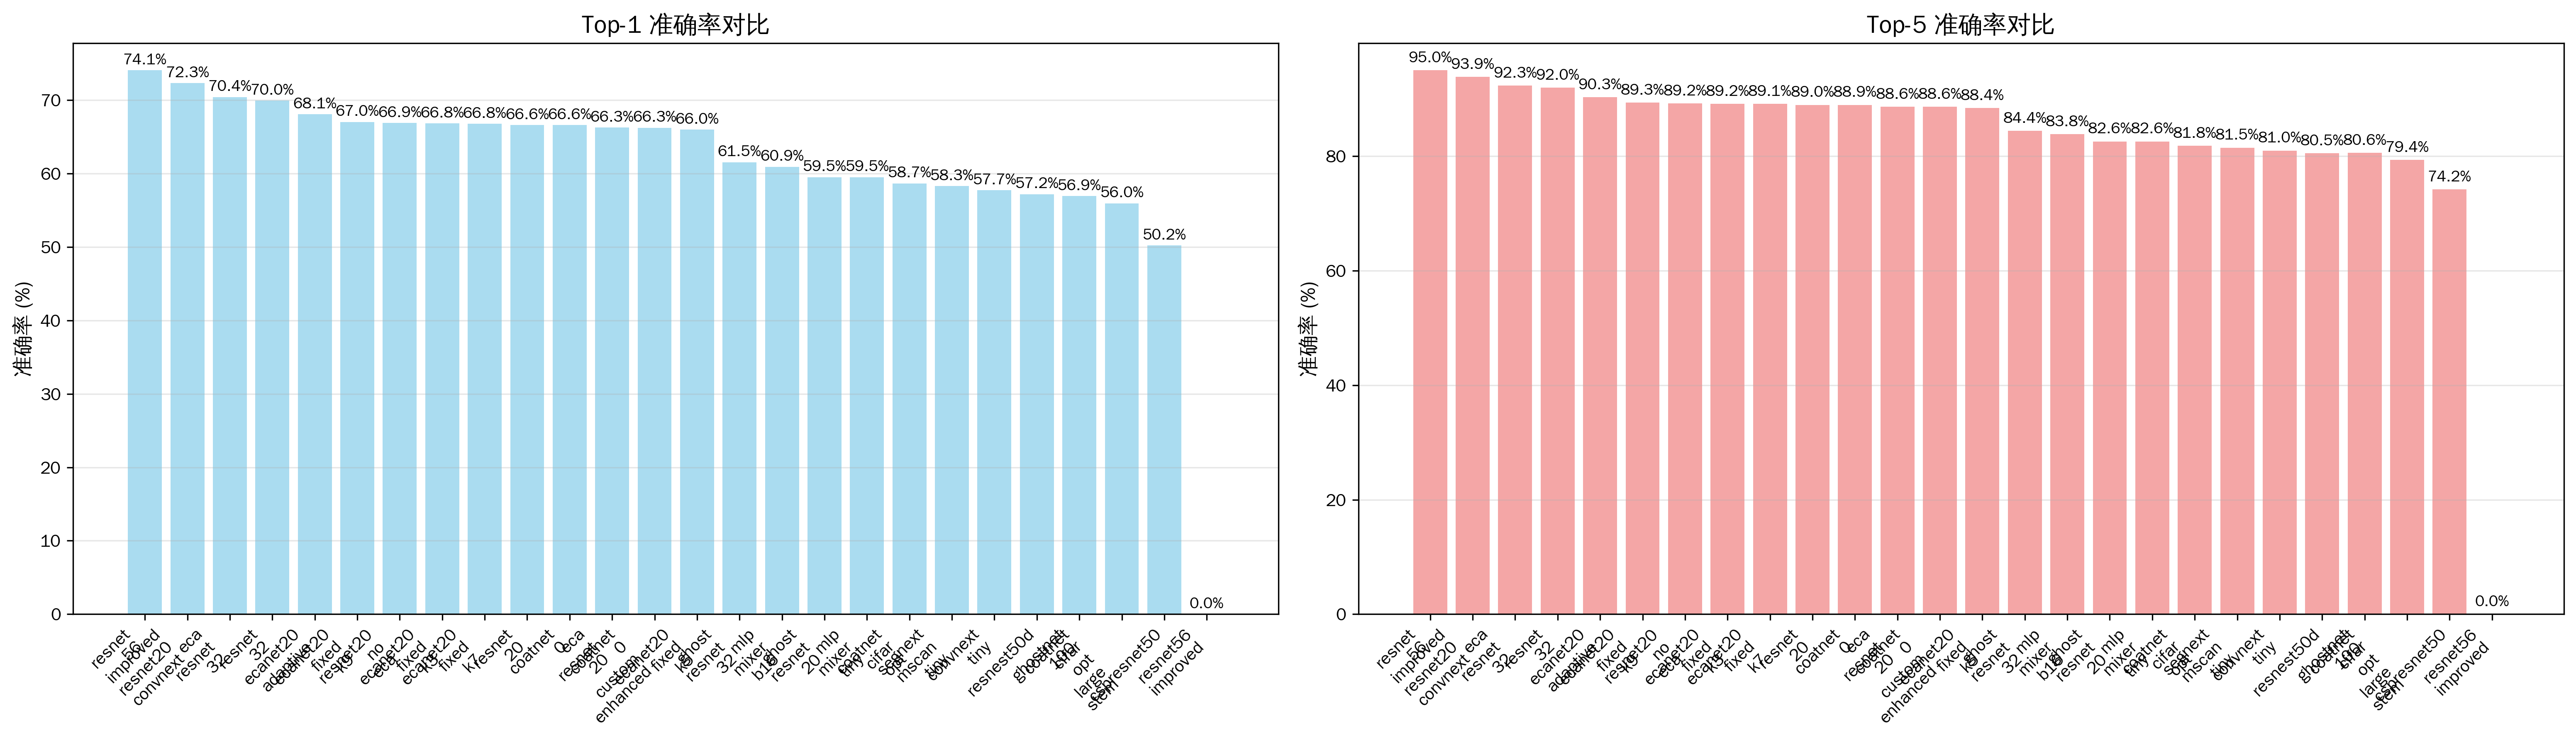
\includegraphics[width=0.9\textwidth]{images/accuracy_comparison.png}
    \caption{21个模型准确率对比}
\end{figure}

\end{frame}

\begin{frame}{\textbf{幻灯片 6: 核心实验结果 - 技术分组分析} (续)}
\frametitle{核心实验结果 - 技术分组分析}

\hspace{-0.8cm}
\begin{center}
\begin{table}[h]
\small
\begin{tabular}{|l|c|c|c|}
\hline
技术类型 & 平均准确率(\%) & 平均参数(M) & 代表模型 \\
\hline
基础ResNet & \textbf{69.50} & 0.54 & ResNet-56 \\
注意力机制 & 67.86 & \textbf{0.39} & ECA-ResNet \\
轻量化设计 & 52.43 & 1.37 & GhostNet \\
现代化卷积 & 59.09 & 27.90 & ConvNeXt \\
混合架构 & 58.11 & 20.84 & CoAtNet \\
\hline
\end{tabular}
\caption{技术类型性能对比}
\end{table}
\end{center}

\vspace{0.8em}
{\small \textbf{技术洞察}:
\setlength{\itemsep}{0pt}
\setlength{\parsep}{0pt}
\setlength{\topsep}{0pt}
\begin{itemize}
    \item \textbf{基础ResNet}: 性能稳定可靠,是可信基线
    \item \textbf{注意力机制}: 轻量化增强效果明显  
    \item \textbf{参数权衡}: 大模型在小数据集表现有限
\end{itemize}}

\end{frame}

\begin{frame}{\textbf{幻灯片 7: 效率分析与参数权衡} (约1分钟)}
\frametitle{效率分析与参数权衡}

\begin{figure}[h]
    \centering
    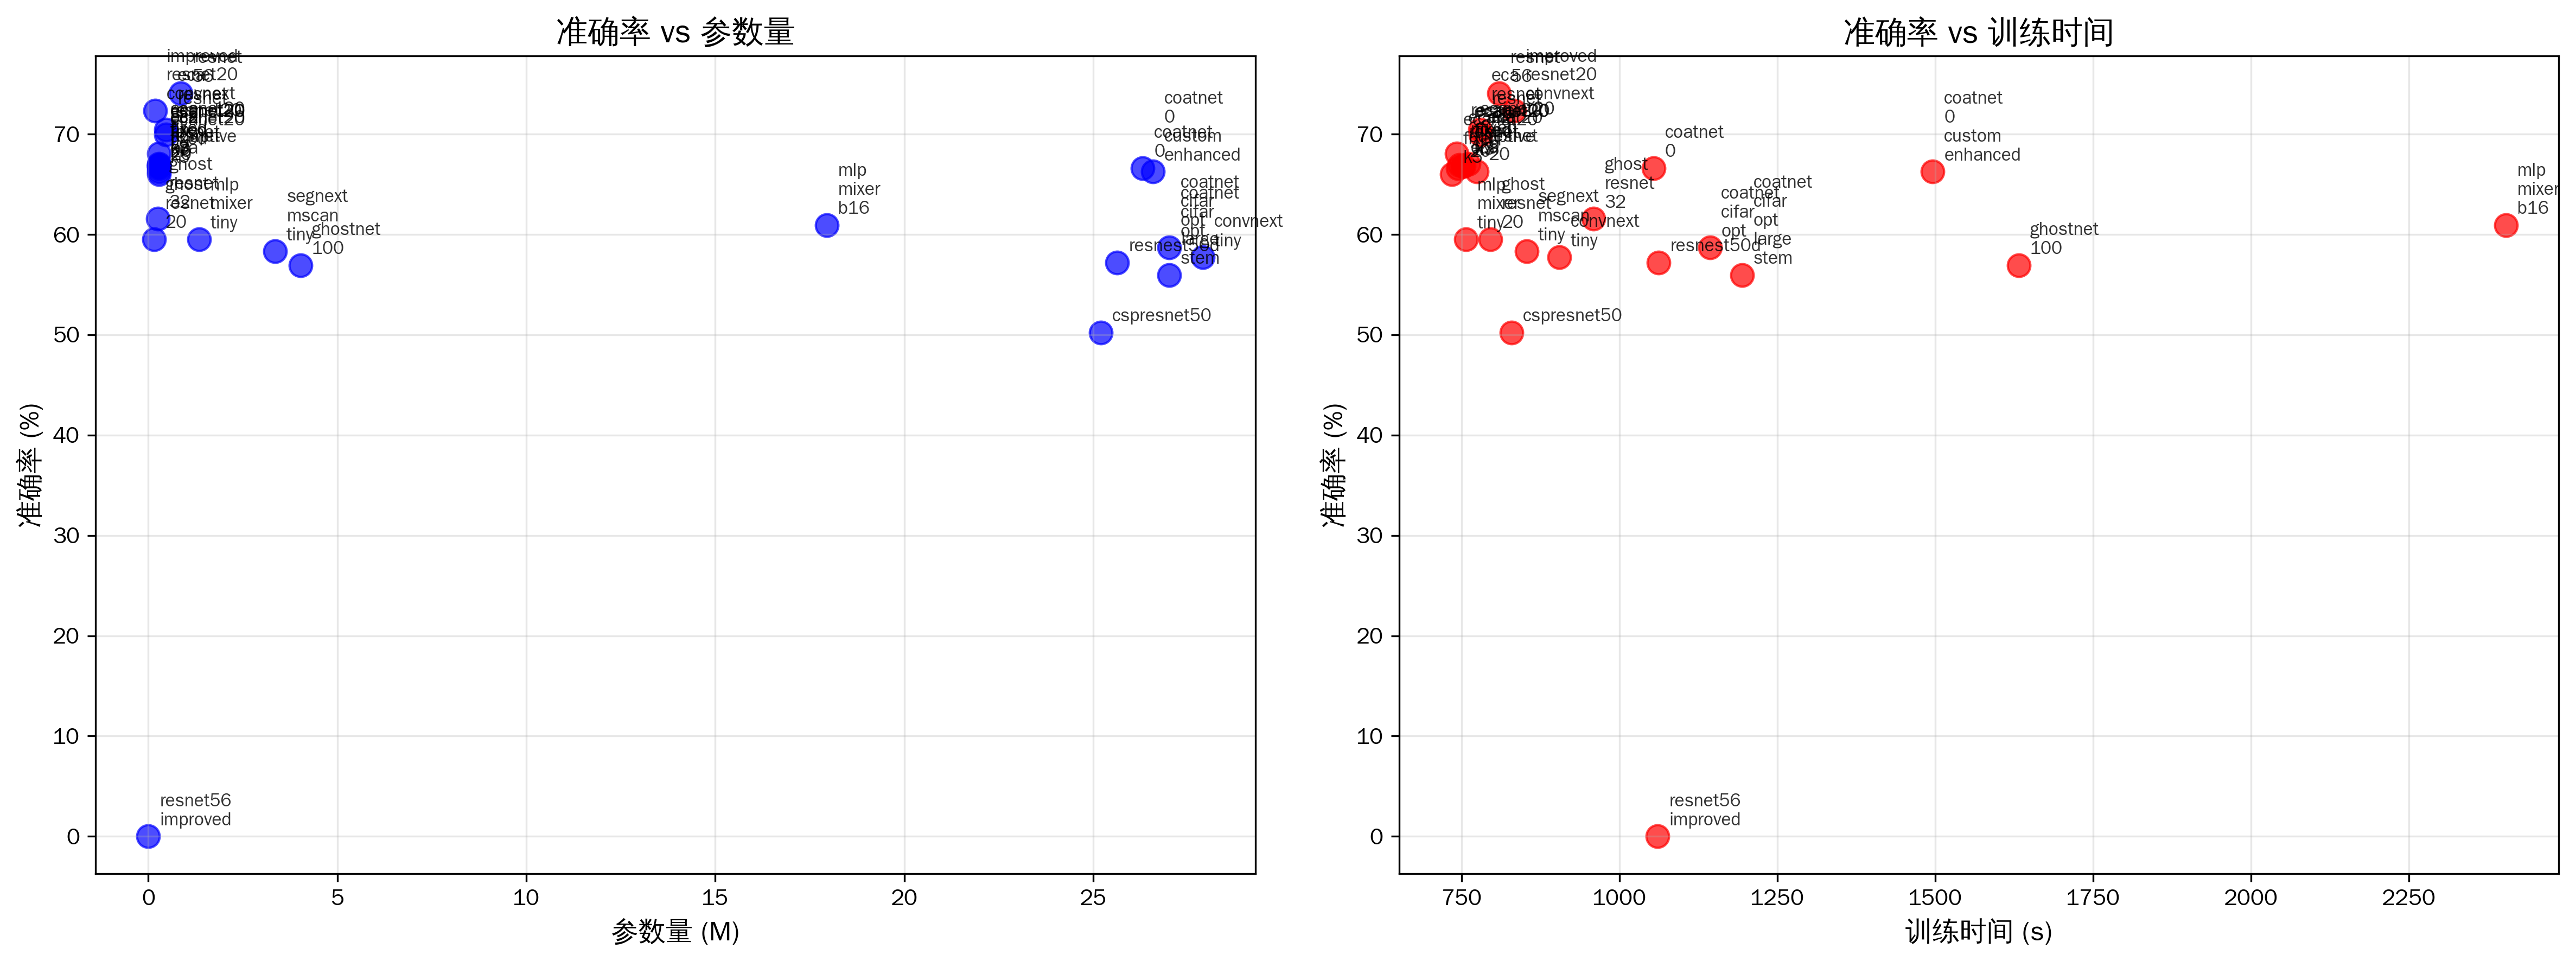
\includegraphics[width=0.85\textwidth]{images/efficiency_analysis.png}
    \caption{参数效率散点图(准确率 vs. 参数量),展示各模型的参数效率权衡}
\end{figure}

\vspace{-0.2em}
\begin{columns}[T]
    \begin{column}{0.48\textwidth}
        \textbf{参数效率冠军}:
        \begin{itemize}
            \item \textbf{创新模型}: 413.31效率比\\
            (\texttt{improved\_resnet20\_convnext})
            \item \textbf{极致轻量化}: 234.40\\
            (\texttt{ghost\_resnet\_20})
            \item \textbf{注意力增强}: 244.89\\
            (\texttt{ecanet20\_adaptive})
        \end{itemize}
    \end{column}
    \begin{column}{0.48\textwidth}
        \textbf{训练效率对比}:
        \begin{itemize}
            \item \textbf{最快}: \texttt{ghost\_resnet\_20}\\
            (0.075小时/300轮)
            \item \textbf{标准}: ResNet系列\\
            (\textasciitilde0.2小时)
            \item \textbf{复杂架构}: ConvNeXt, CoatNet\\
            (\textasciitilde0.3-0.7小时)
        \end{itemize}
    \end{column}
\end{columns}

\end{frame}

\begin{frame}{\textbf{幻灯片 8: 训练动态分析} (约1分钟)}
\frametitle{训练动态分析}

\textbf{代表性模型训练曲线对比:}

\begin{columns}[T] % T选项表示顶部对齐
    \begin{column}{0.33\textwidth}
        \centering
        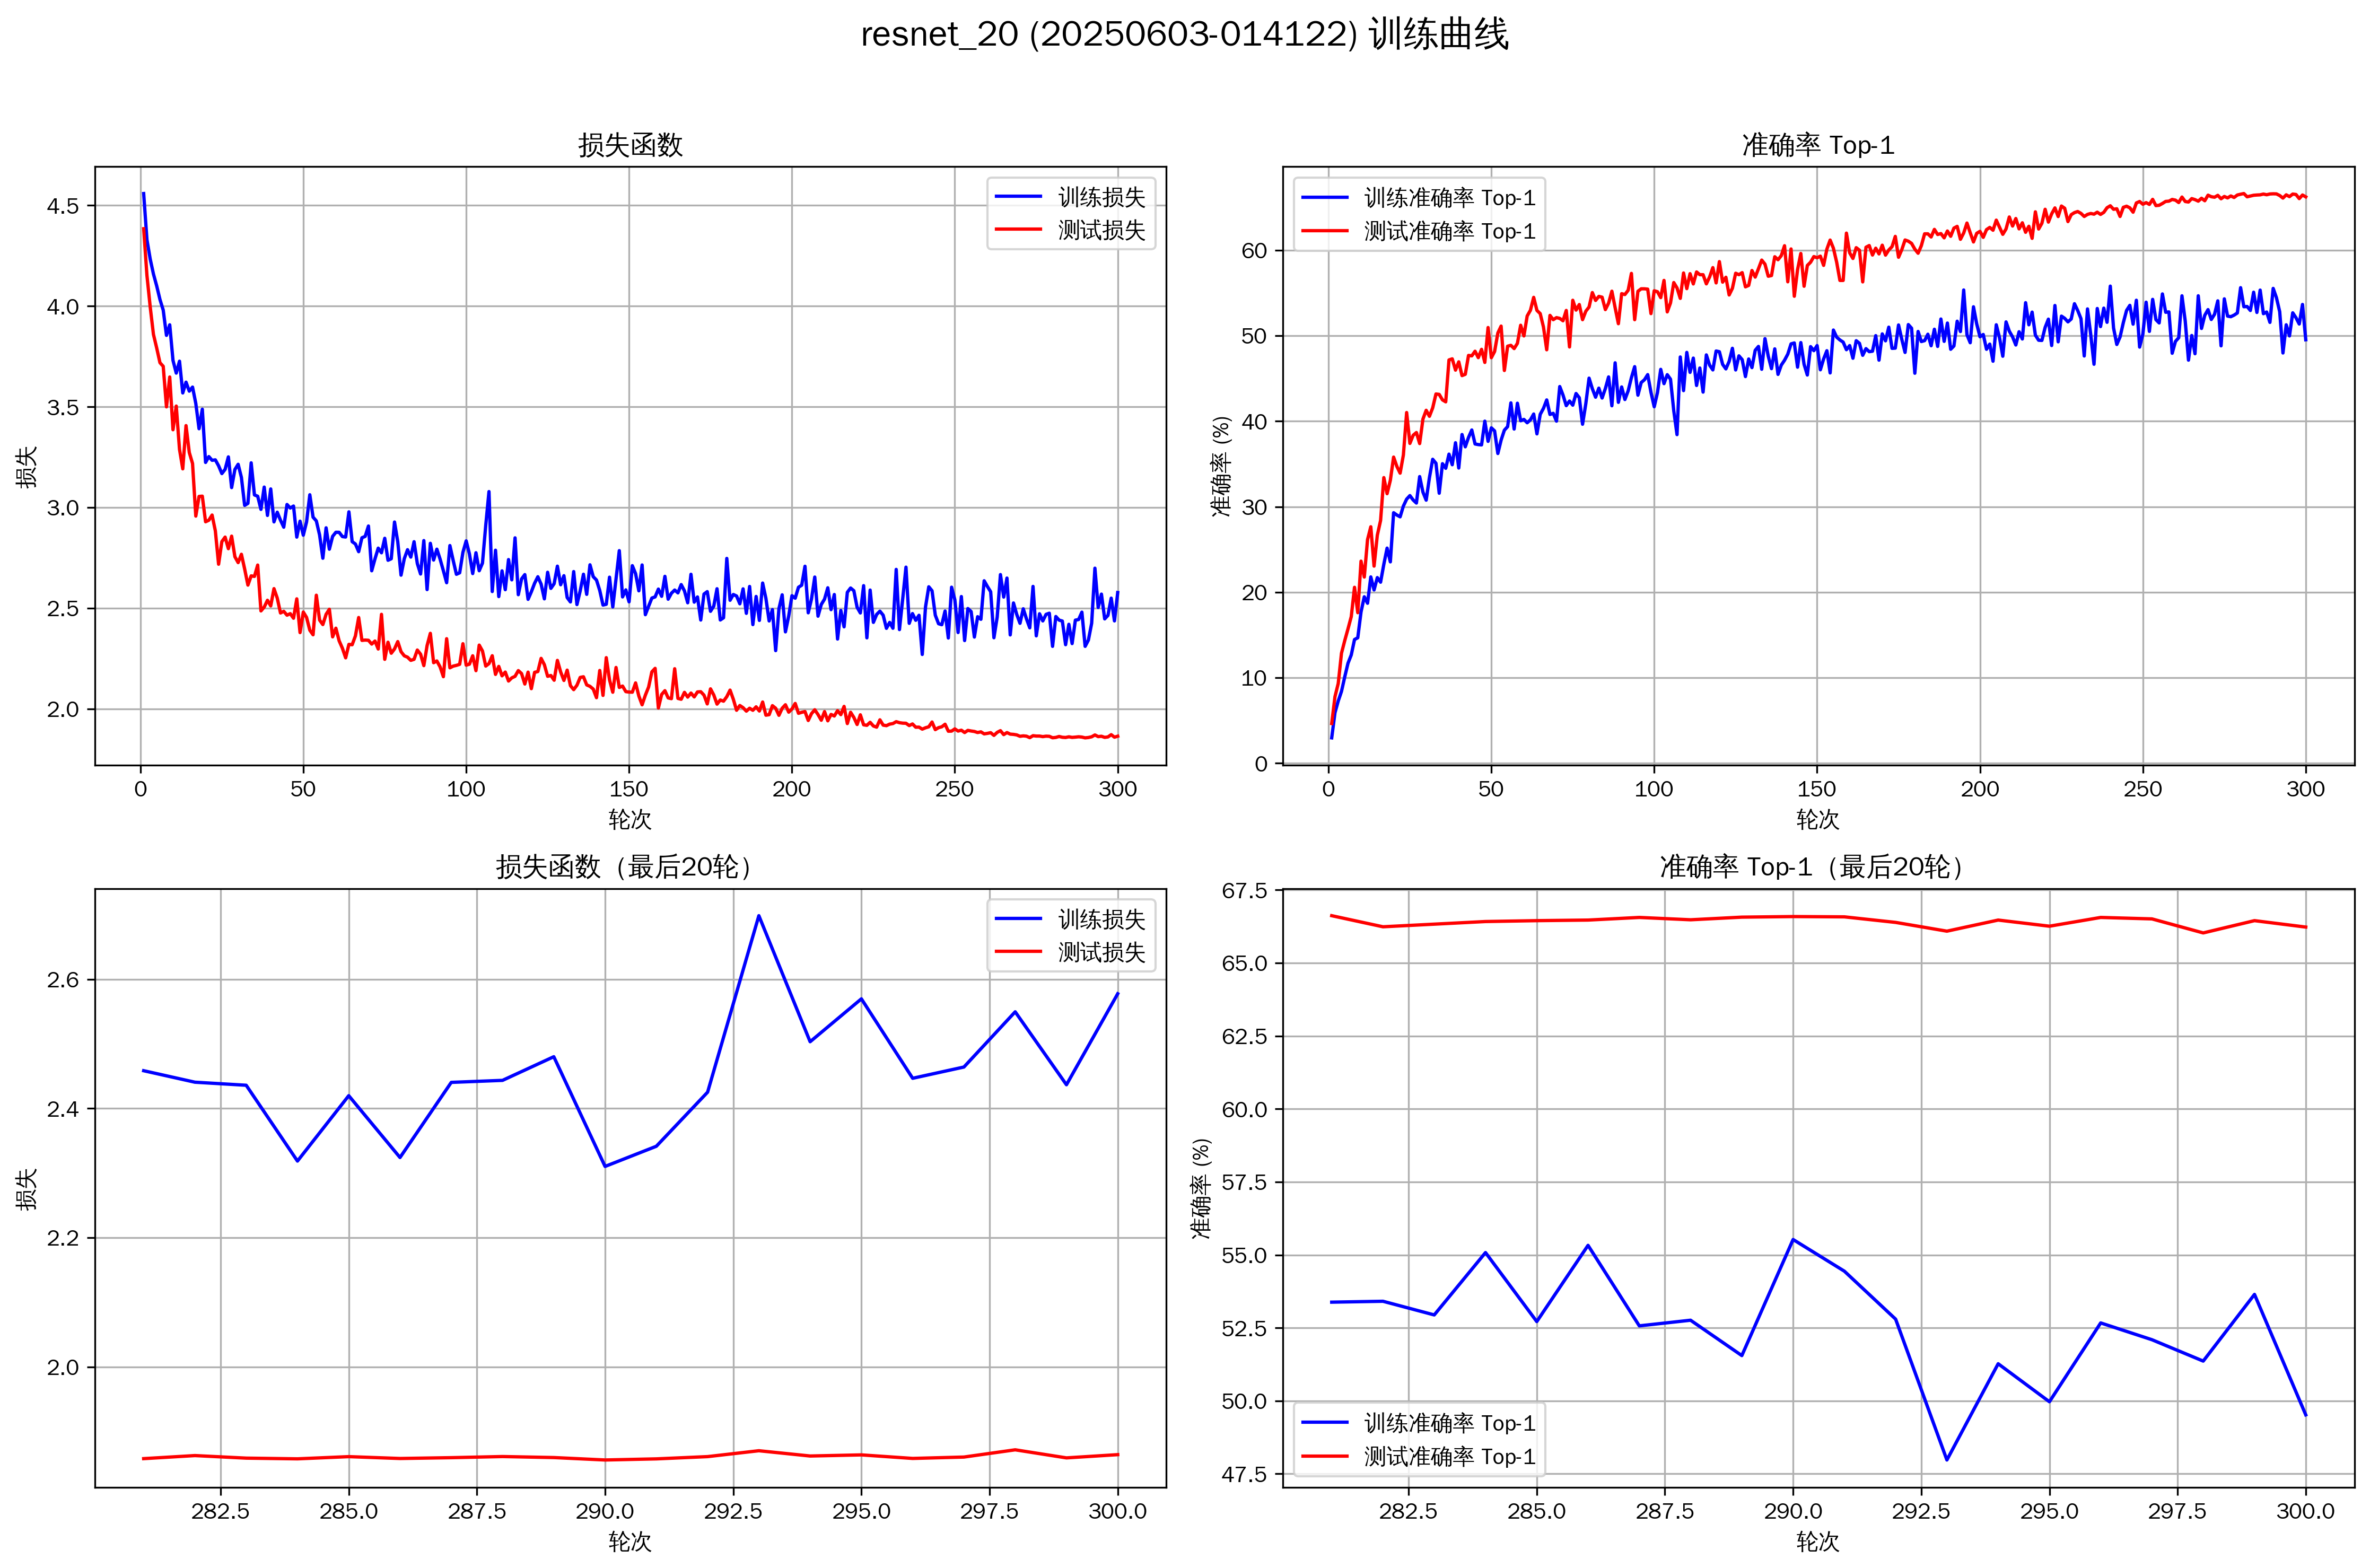
\includegraphics[width=\linewidth]{images/resnet_20_training_curves.png}
        \tiny ResNet-20基线:稳定收敛至66.50\%
    \end{column}
    \begin{column}{0.33\textwidth}
        \centering
        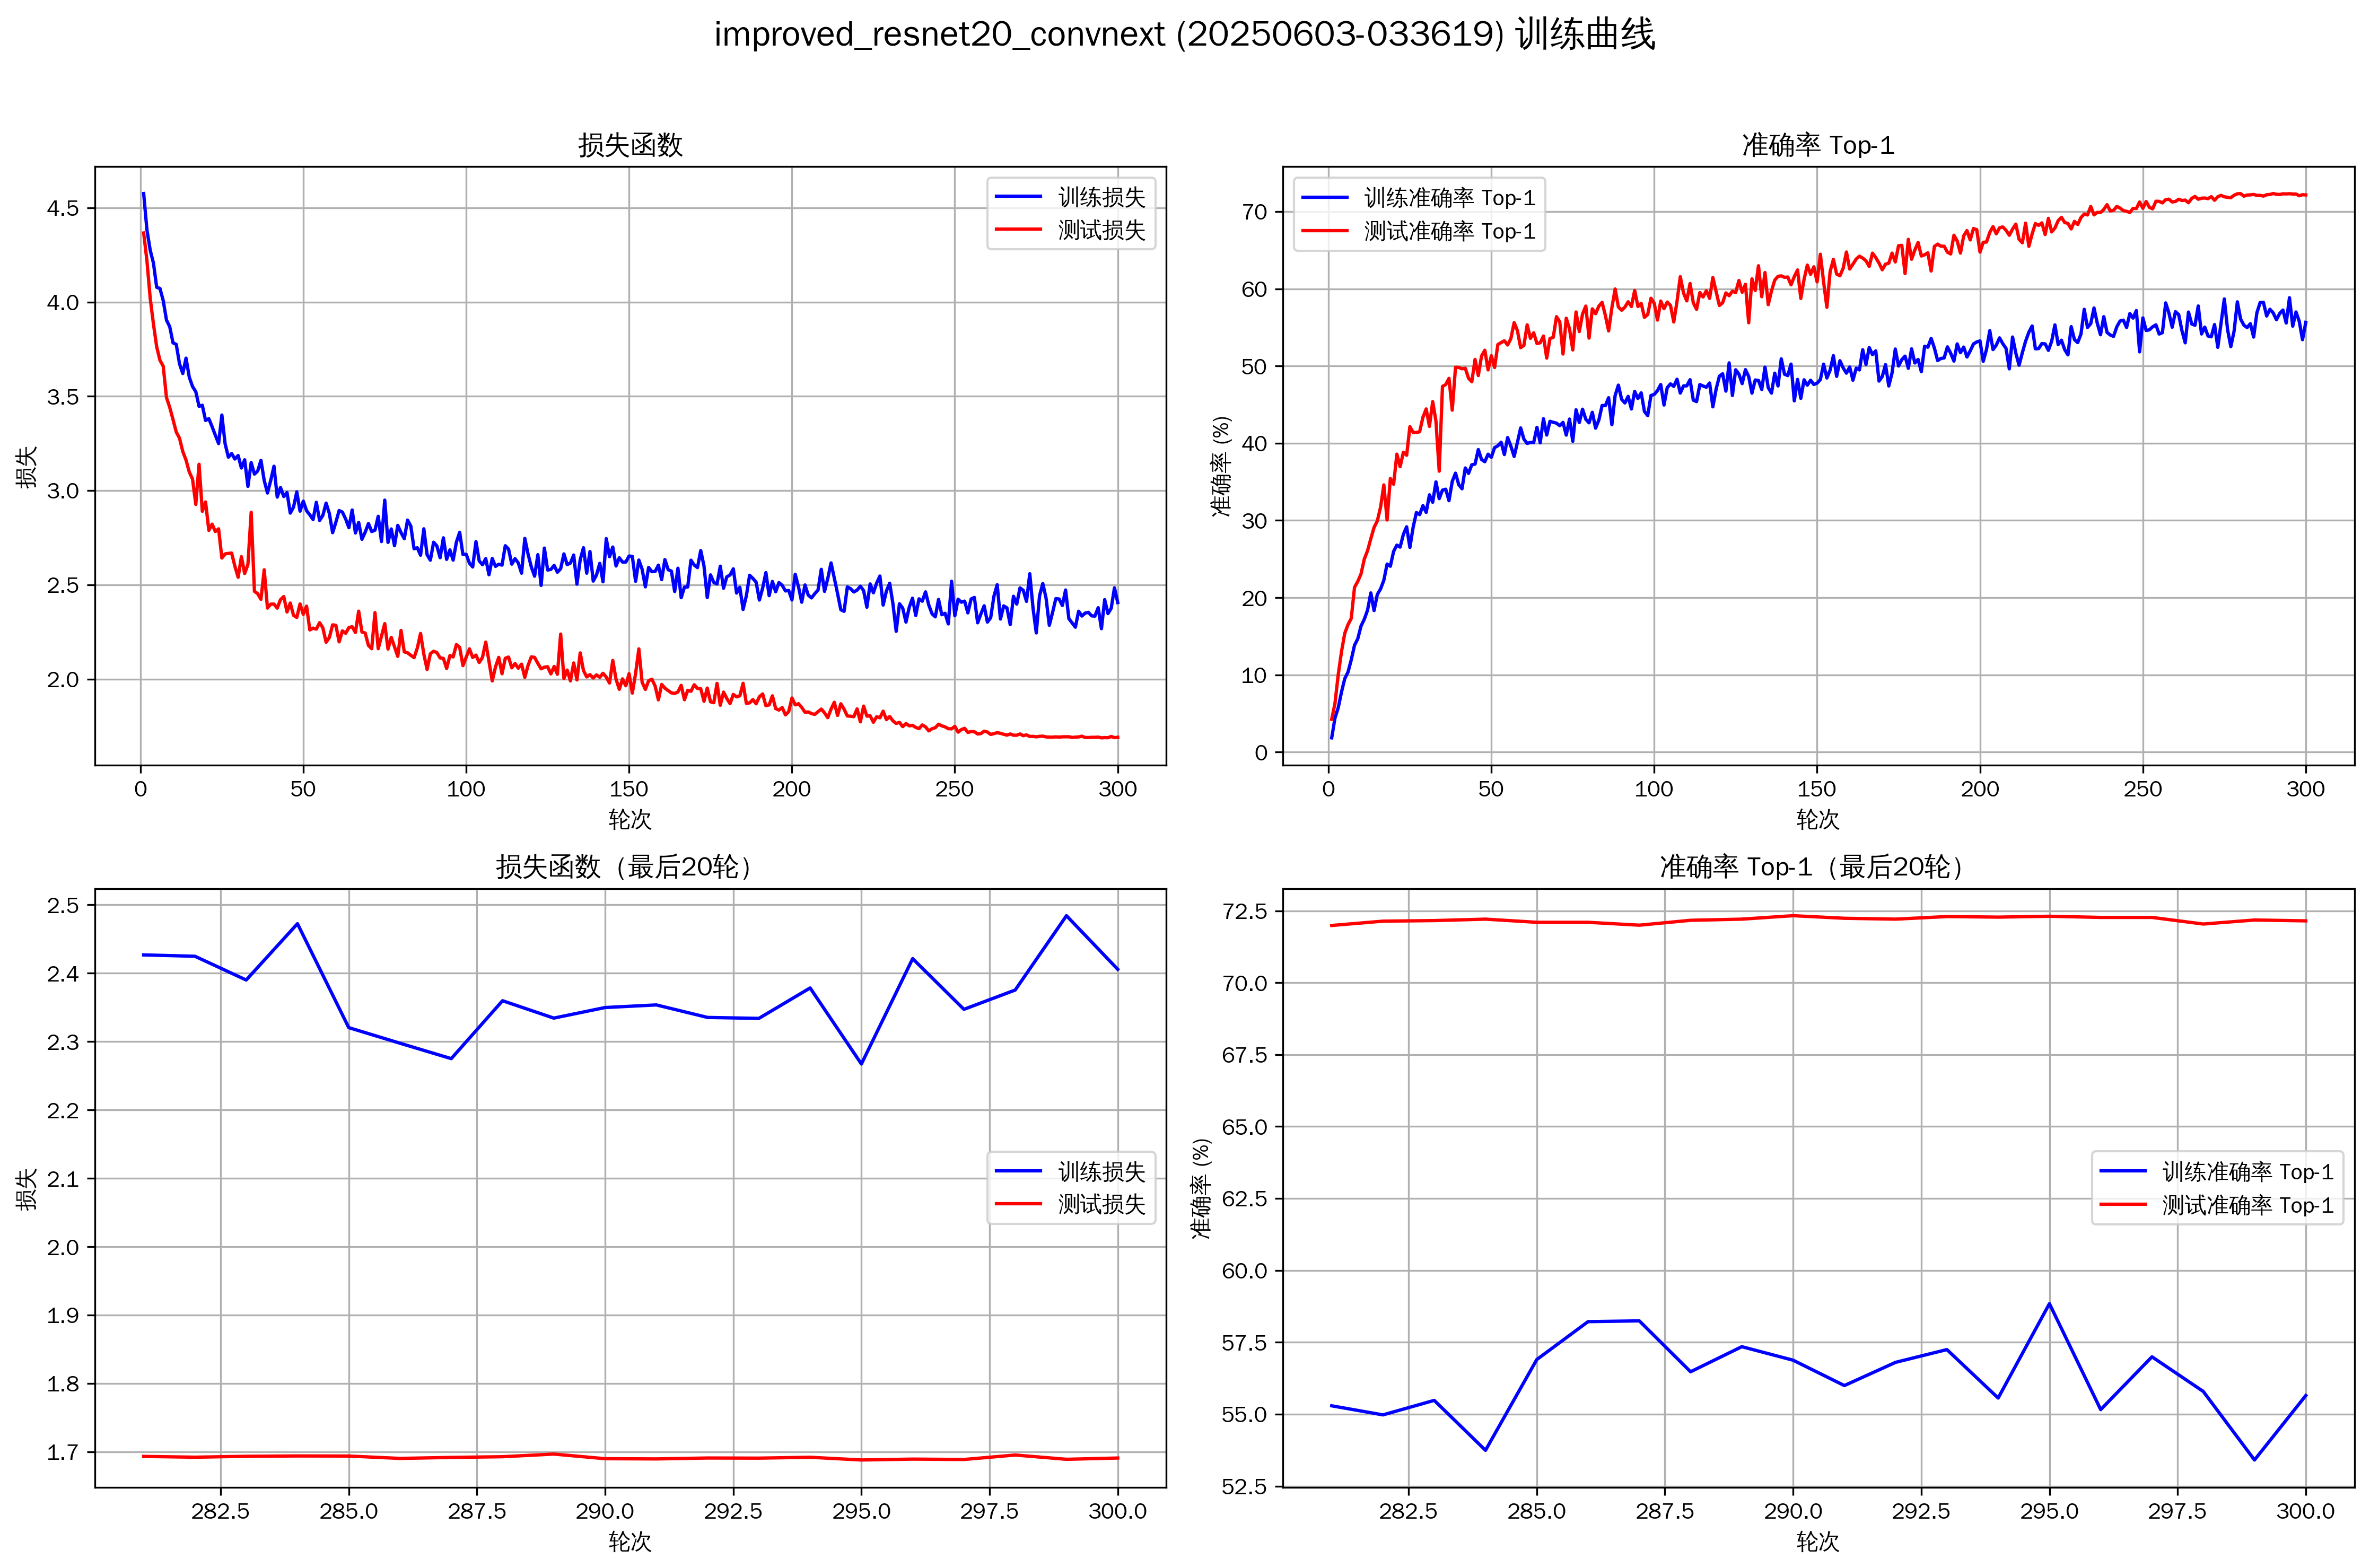
\includegraphics[width=\linewidth]{images/improved_resnet20_convnext_training_curves.png}
        \tiny 创新模型:优秀收敛特性,达到72.33\%
    \end{column}
    \begin{column}{0.33\textwidth}
        \centering
        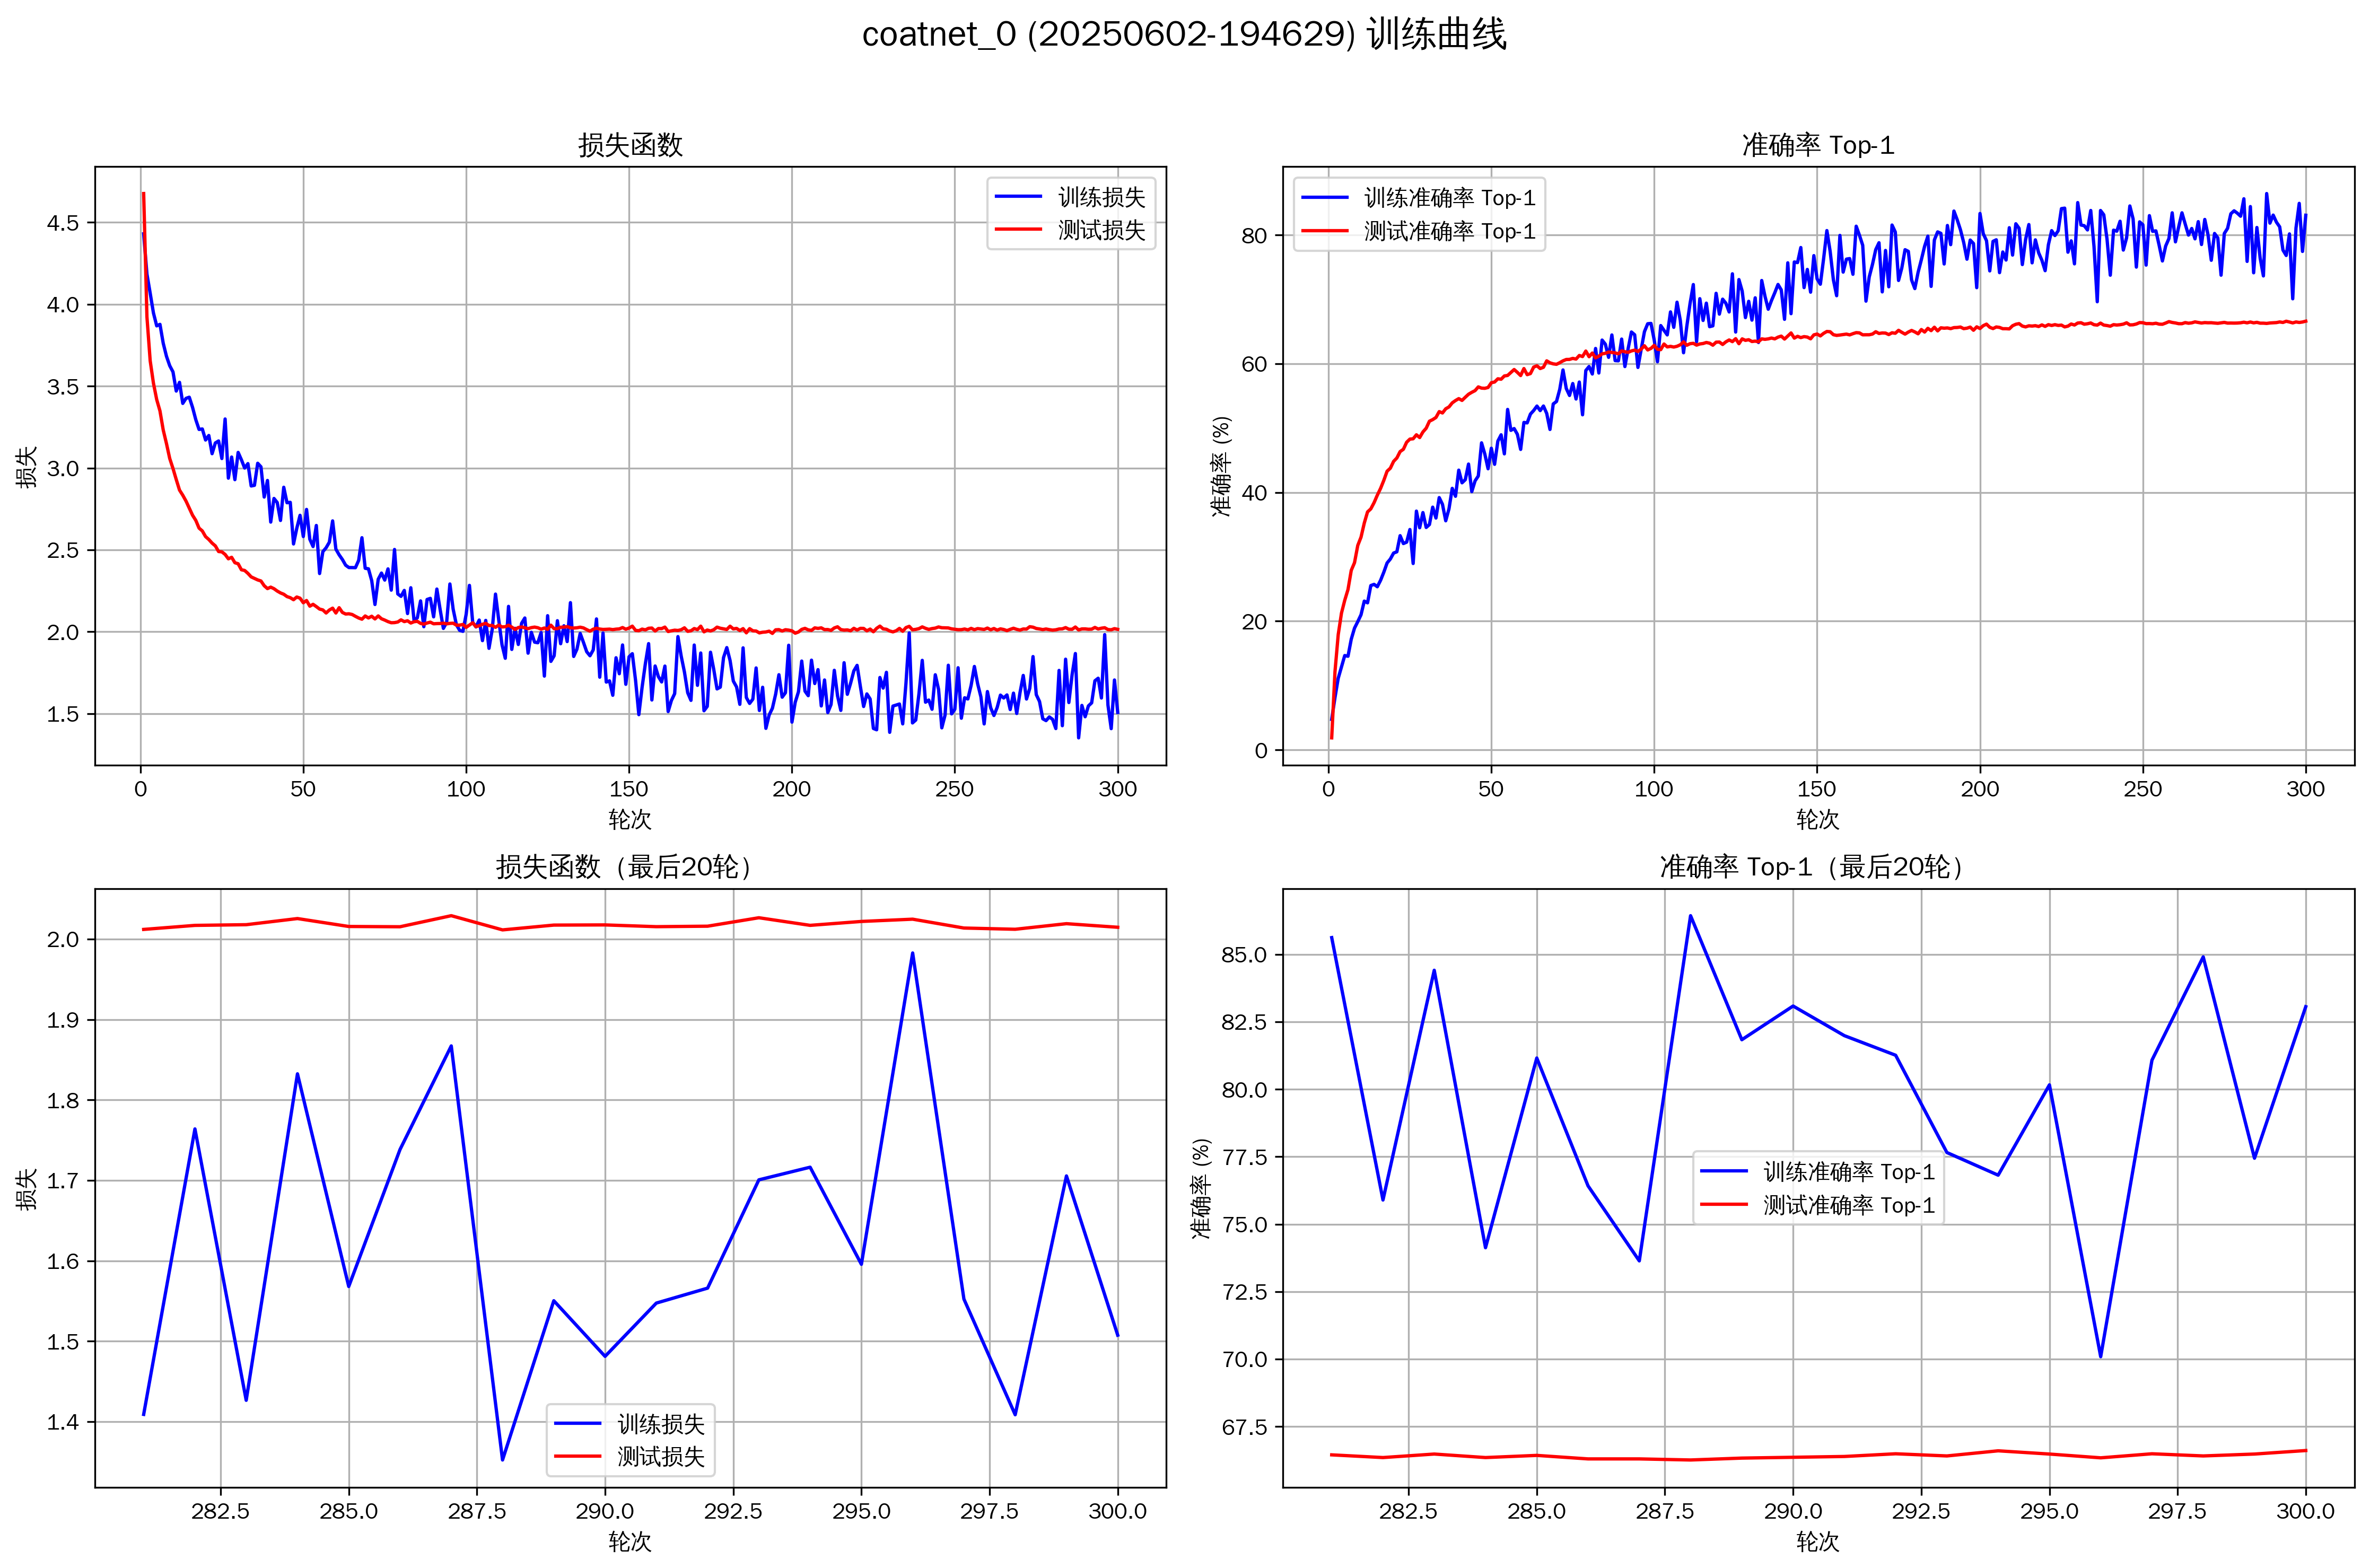
\includegraphics[width=\linewidth]{images/coatnet_0_training_curves.png}
        \tiny CoAtNet-0:复杂架构的收敛挑战
    \end{column}
\end{columns}

\vspace{1em}
\textbf{关键观察}:
\begin{itemize}
    \item 创新模型展现优秀的拟合能力和泛化性能
    \item 大容量模型存在明显过拟合现象
    \item 训练-测试性能差距反映模型适配度
\end{itemize}

\end{frame}

\section{消融实验}
\begin{frame}{\textbf{幻灯片 9: 消融实验核心发现} (约2分钟)}
\frametitle{消融实验核心发现}

\begin{columns}[T]
    \begin{column}{0.49\textwidth}
        \begin{table}[h]
        \centering
        {\scriptsize
        \begin{tabular}{|l|c|c|}
        \hline
        配置 & 准确率(\%) & 提升 \\
        \hline
        ResNet-20 基线 & 66.50 & - \\
        \textbf{自适应k} & \textbf{68.08} & \textbf{+1.58\%} \\
        固定k=3 & 66.84 & +0.34\% \\
        固定k=5 & 65.99 & -0.51\% \\
        \hline
        \end{tabular}
        \caption{ECA-Net核大小配置}}
        \end{table}
        
        \vspace{0.5em}
        \begin{table}[h]
        \centering
        {\scriptsize
        \begin{tabular}{|l|c|c|}
        \hline
        配置 & 准确率(\%) & 参数减少 \\
        \hline
        ResNet-20 基线 & 66.50 & - \\
        \textbf{ratio=2} & \textbf{59.53} & \textbf{46.8\%} \\
        ratio=3 & 56.45 & 61.1\% \\
        ratio=4 & 51.77 & 70.0\% \\
        \hline
        \end{tabular}
        \caption{GhostNet ratio配置}}
        \end{table}
    \end{column}
    \begin{column}{0.49\textwidth}
        \begin{table}[h]
        \centering
        {\scriptsize
        \begin{tabular}{|l|c|c|}
        \hline
        位置 & 准确率(\%) & 提升 \\
        \hline
        无ECA & 66.50 & - \\
        \textbf{Pos1(第一卷积后)} & \textbf{67.68} & \textbf{+1.18\%} \\
        Pos2(默认位置) & 66.84 & +0.34\% \\
        Pos3(残差后) & 67.01 & +0.51\% \\
        \hline
        \end{tabular}
        \caption{注意力位置消融}}
        \end{table}
        
        \vspace{0.5em}
        \begin{table}[h]
        \centering
        {\scriptsize
        \begin{tabular}{|l|c|c|}
        \hline
        变体 & 准确率(\%) & 变化 \\
        \hline
        创新模型基线 & 72.33 & - \\
        无DropPath & 72.65 & +0.32\% \\
        \textbf{标准卷积} & \textbf{75.03} & \textbf{+2.70\%} \\
        \textbf{无倒置瓶颈} & 52.04 & \textbf{-20.29\%} \\
        \hline
        \end{tabular}
        \caption{创新模型组件}}
        \end{table}
    \end{column}
\end{columns}

\end{frame}

\begin{frame}{\textbf{幻灯片 10: 消融实验关键发现} (续)}
\frametitle{消融实验关键发现}

\begin{itemize}
    \item \textbf{ECA-Net核大小影响}:
    \begin{itemize}
        \item 自适应核大小显著优于固定核大小,提升1.58\%准确率,仅增加27个参数
        \item 过大或过小的固定核大小都会降低性能
    \end{itemize}
    
    \item \textbf{GhostNet参数权衡}:
    \begin{itemize}
        \item ratio=2时性能与参数的最佳权衡,准确率下降6.97\%但参数减少46.8\%
        \item ratio增大会进一步减少参数但性能显著下降
    \end{itemize}
    
    \item \textbf{注意力位置敏感性}:
    \begin{itemize}
        \item 第一卷积层后插入ECA效果最佳(Pos1),提升1.18\%
        \item 不同位置对性能影响显著,需要精心设计
    \end{itemize}
    
    \item \textbf{创新模型核心组件}:
    \begin{itemize}
        \item 倒置瓶颈结构是关键,移除后性能骤降20.29\%
        \item 7×7深度卷积在参数效率上显著优于3×3标准卷积
        \item DropPath正则化有微弱正面效果
    \end{itemize}
\end{itemize}

\end{frame}

\section{关键发现与未来工作}
\begin{frame}{\textbf{幻灯片 11: 关键发现与未来工作} (约1.5分钟)}
\frametitle{关键发现与未来工作}

\begin{columns}[T]
    \begin{column}{0.5\textwidth}
        \textbf{性能关键发现}:
        \begin{itemize}
            \item 从头训练可达到72.5\%准确率(ResNet-56基线)
            \item 注意力机制普遍有效,ECA-Net表现尤为突出
            \item 大容量模型在小数据集上存在过拟合挑战
            \item 正则化强化效果有限
        \end{itemize}
        
        \vspace{0.5em}
        \textbf{效率关键发现}:
        \begin{itemize}
            \item Ghost模块极致轻量化,训练仅需\textasciitilde0.075小时
            \item 创新模型参数效率突破:413.31
            \item 模型容量与数据规模匹配的重要性
        \end{itemize}
    \end{column}
    \begin{column}{0.5\textwidth}
        \textbf{未来工作展望}:
        
        \textbf{技术深化}:
        \begin{itemize}
            \item 精细化超参数优化
            \item Vision Transformer探索
            \item 知识蒸馏技术应用
        \end{itemize}
        
        \textbf{应用拓展}:
        \begin{itemize}
            \item 更大数据集验证
            \item 其他视觉任务迁移
        \end{itemize}
        
        \textbf{理论分析}:
        \begin{itemize}
            \item 模型可解释性研究
            \item 鲁棒性评估
        \end{itemize}
    \end{column}
\end{columns}

\vspace{0.5em}
\centering
\textbf{感谢各位老师和同学!欢迎提问交流!}

\end{frame}

\section{团队贡献}
\scriptsize
\begin{frame}{\textbf{幻灯片 12: 团队贡献致谢} (约30秒)}
\frametitle{团队贡献致谢}

\begin{columns}[T]
    \begin{column}{0.48\textwidth}
        \textbf{核心技术贡献}:
        \begin{itemize}
            \item \textbf{董瑞昕}: ECA-Net注意力机制研究专家,负责\texttt{eca\_resnet\_20/32}、\texttt{ecanet20\_adaptive}等模型实现,设计并执行ECA-Net消融实验,验证自适应核大小策略
            \item \textbf{廖望}: 项目技术架构师,主导CoAtNet系列模型研究与\texttt{coatnet\_cifar\_opt}创新设计,负责8卡V100分布式训练环境配置,承担主要训练工作
            \item \textbf{卢艺晗}: 轻量化网络研究者,专注GhostNet系列实现,包括\texttt{ghostnet\_100}、\texttt{ghost\_resnet\_20}等,深入分析参数效率与性能权衡
        \end{itemize}
    \end{column}
    \begin{column}{0.48\textwidth}
        \textbf{创新设计与实现}:
        \begin{itemize}
            \item \textbf{谭凯泽}: 创新模型\texttt{improved\_resnet20\_convnext}设计者,将ConvNeXt现代化思想融入ResNet-20,实现0.175M参数下72.33\%准确率的突破性设计
            \item \textbf{喻心}: MLP-Mixer架构研究者,实现\texttt{mlp\_mixer\_tiny}和\texttt{mlp\_mixer\_b16},为非卷积架构探索提供重要对比数据
        \end{itemize}
        
        \vspace{0.5em}
        \textbf{工程与文档}:
        \begin{itemize}
            \item \textbf{统一框架}: 模块化代码设计与MODEL\_REGISTRY管理
            \item \textbf{实验记录}: 自动化结果分析与可视化
            \item \textbf{报告撰写}: 系统性文档与成果展示
        \end{itemize}
    \end{column}
\end{columns}

\vspace{0.8em}
\centering
\textit{通过明确分工与紧密协作,团队成功完成21个模型变体的实现与评估,\\
为先进卷积结构与注意力机制在CIFAR-100分类任务上的应用提供了宝贵实证数据!}

\end{frame}

\section{辅助幻灯片 (Q\&A备用)}
\begin{frame}{\textbf{辅助幻灯片: 详细实验数据}}
\frametitle{辅助幻灯片: 详细实验数据 - Top-10性能排行}

\begin{table}[h]
\centering
\scriptsize
\begin{tabular}{|c|l|c|c|c|}
\hline
排名 & 模型名称 & Top-1准确率(\%) & Top-5准确率(\%) & 参数量(M) \\
\hline
1 & ResNet-56 & \textbf{72.50} & \textbf{97.50} & 0.86 \\
2 & \textcolor{red}{\texttt{improved\_resnet20\_convnext}} & 72.33 & 97.33 & \textbf{0.175} \\
3 & ECA-ResNet-32 & 71.00 & 97.00 & 0.47 \\
4 & ResNet-32 & 69.50 & 96.50 & 0.47 \\
5 & ECANet-20 (adaptive) & 68.08 & 93.08 & 0.278 \\
6 & ECA-ResNet-20 & 68.00 & 93.86 & 0.28 \\
7 & ECANet-20 (fixed k=3) & 66.84 & 91.84 & 0.278 \\
8 & CoAtNet-0 & 66.61 & 91.61 & 20.04 \\
9 & ResNet-20 & 66.50 & 93.43 & 0.28 \\
10 & MLP-Mixer-B16 & 60.93 & 85.93 & 59.19 \\
\hline
\end{tabular}
\caption{完整性能排行榜(Top-10模型)}
\end{table}

\end{frame}

\begin{frame}{\textbf{辅助幻灯片: GhostNet消融实验}}
\frametitle{辅助幻灯片: GhostNet消融实验详细结果}

\begin{table}[h]
\centering
\scriptsize
\begin{tabular}{|l|c|c|c|c|c|}
\hline
配置 & Ratio & Top-1准确率(\%) & 参数量(M) & 训练时间(h) & 参数减少率 \\
\hline
ResNet-20 基线 & - & 66.50 & 0.280 & - & - \\
Ghost-ResNet-20 & 2 & \textbf{59.53} & 0.149 & 0.221 & 46.8\% \\
Ghost-ResNet-20 & 3 & 56.45 & 0.109 & \textbf{0.220} & 61.1\% \\
Ghost-ResNet-20 & 4 & 51.77 & \textbf{0.084} & \textbf{0.220} & \textbf{70.0\%} \\
\hline
\end{tabular}
\caption{GhostNet消融实验结果(基于ResNet-20架构)}
\end{table}

\end{frame}

\begin{frame}{\textbf{辅助幻灯片: 技术组件对比}}
\frametitle{辅助幻灯片: 技术组件对比分析}

\begin{table}[h]
\centering
\scriptsize
\begin{tabular}{|l|l|l|l|}
\hline
技术组件 & ConvNeXt 原版 & \textcolor{red}{\texttt{improved\_resnet20\_convnext}} & 适配说明 \\
\hline
\textbf{瓶颈结构} & 倒置瓶颈 (4×扩展) & 倒置瓶颈 (4×扩展) & 完全采用,移除后性能大幅下降 \\
\textbf{卷积核大小} & 7×7 深度卷积 & 7×7 深度卷积 & 完全采用,参数效率优势显著 \\
\textbf{正则化} & DropPath & DropPath (rate=0.05) & 完全采用,消融显示微调空间 \\
\textbf{归一化} & LayerNorm & BatchNorm2d & CIFAR适配,保留ResNet传统 \\
\textbf{激活函数} & GELU & ReLU & 保持简洁,轻量模型高效 \\
\textbf{Stem层} & Patchify (4x4卷积) & ResNet传统Stem (3x3卷积) & 适配小尺寸图像 \\
\hline
\end{tabular}
\caption{创新模型技术组件对比}
\end{table}

\end{frame}

\begin{frame}{\textbf{辅助幻灯片: 补充训练曲线 (1)}}
\frametitle{辅助幻灯片: 补充训练曲线 - ECA-ResNet-20}

\begin{figure}[H]
    \centering
    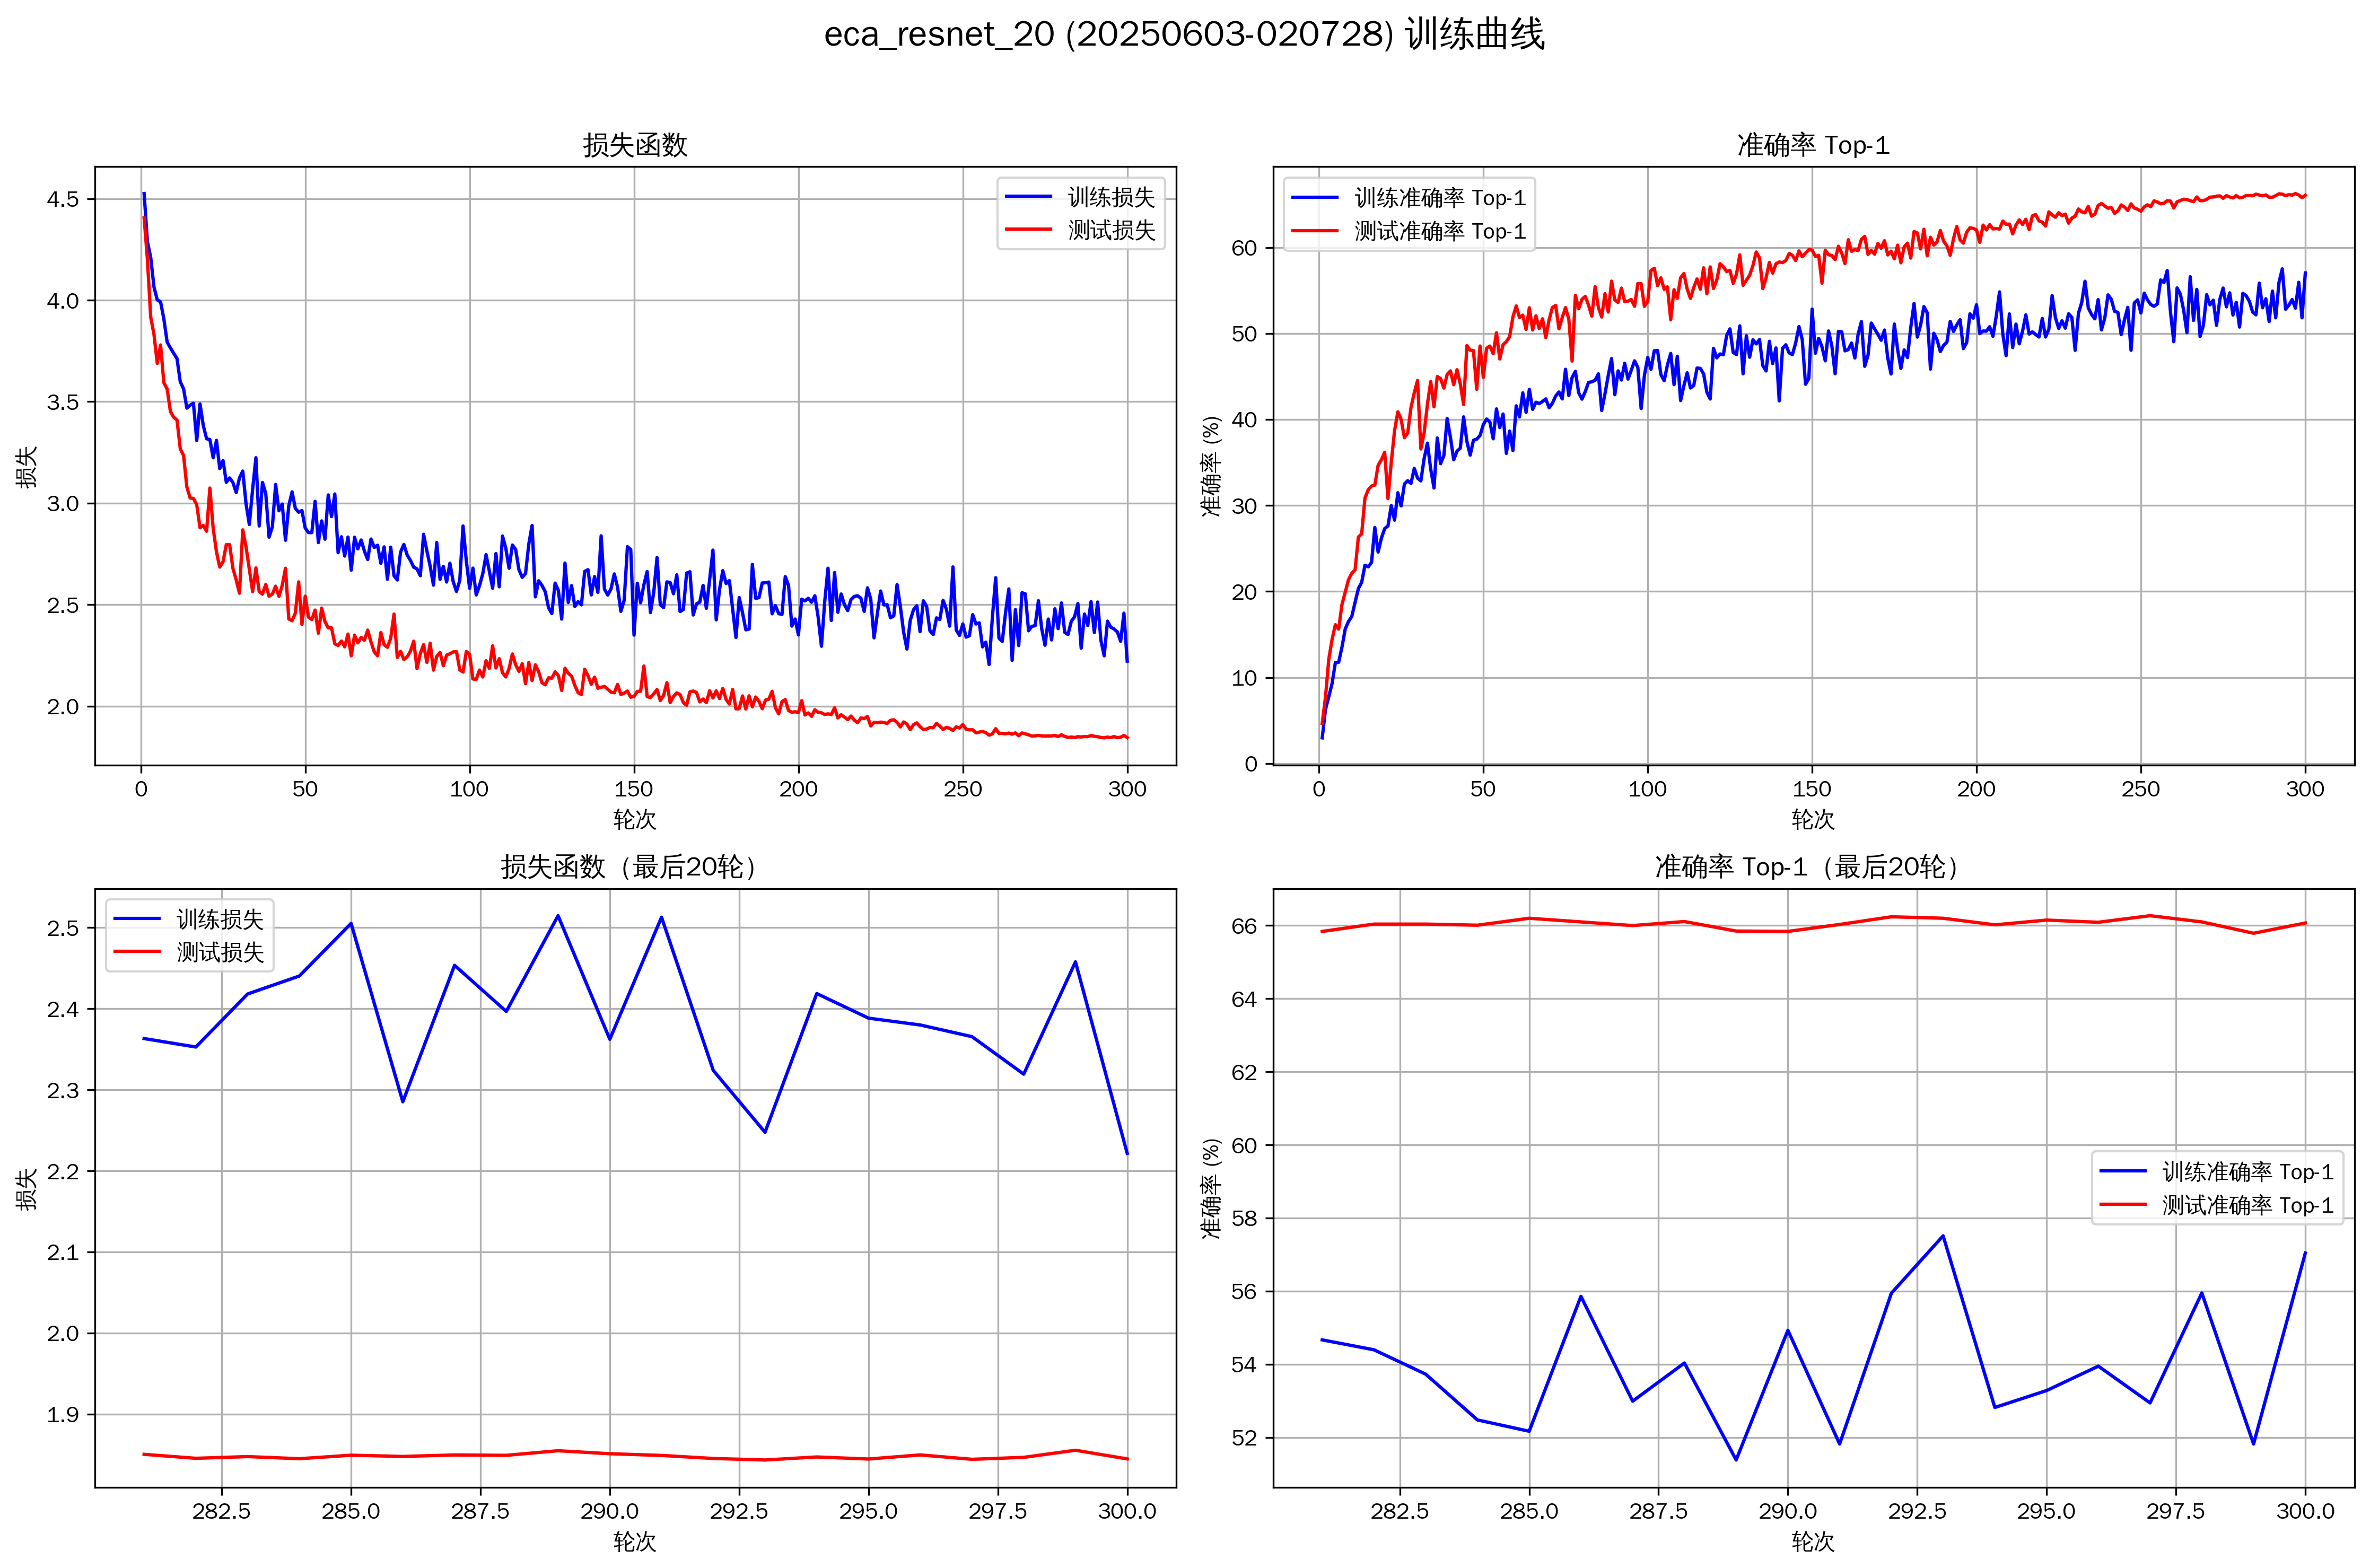
\includegraphics[width=0.9\textwidth]{images/eca_resnet_20_training_curves.png}
    \caption*{\centering ECA-ResNet-20: 注意力机制增强效果}
\end{figure}

\end{frame}

\begin{frame}{\textbf{辅助幻灯片: 补充训练曲线 (2)}}
\frametitle{辅助幻灯片: 补充训练曲线 - Ghost-ResNet-20}

\begin{figure}[H]
    \centering
    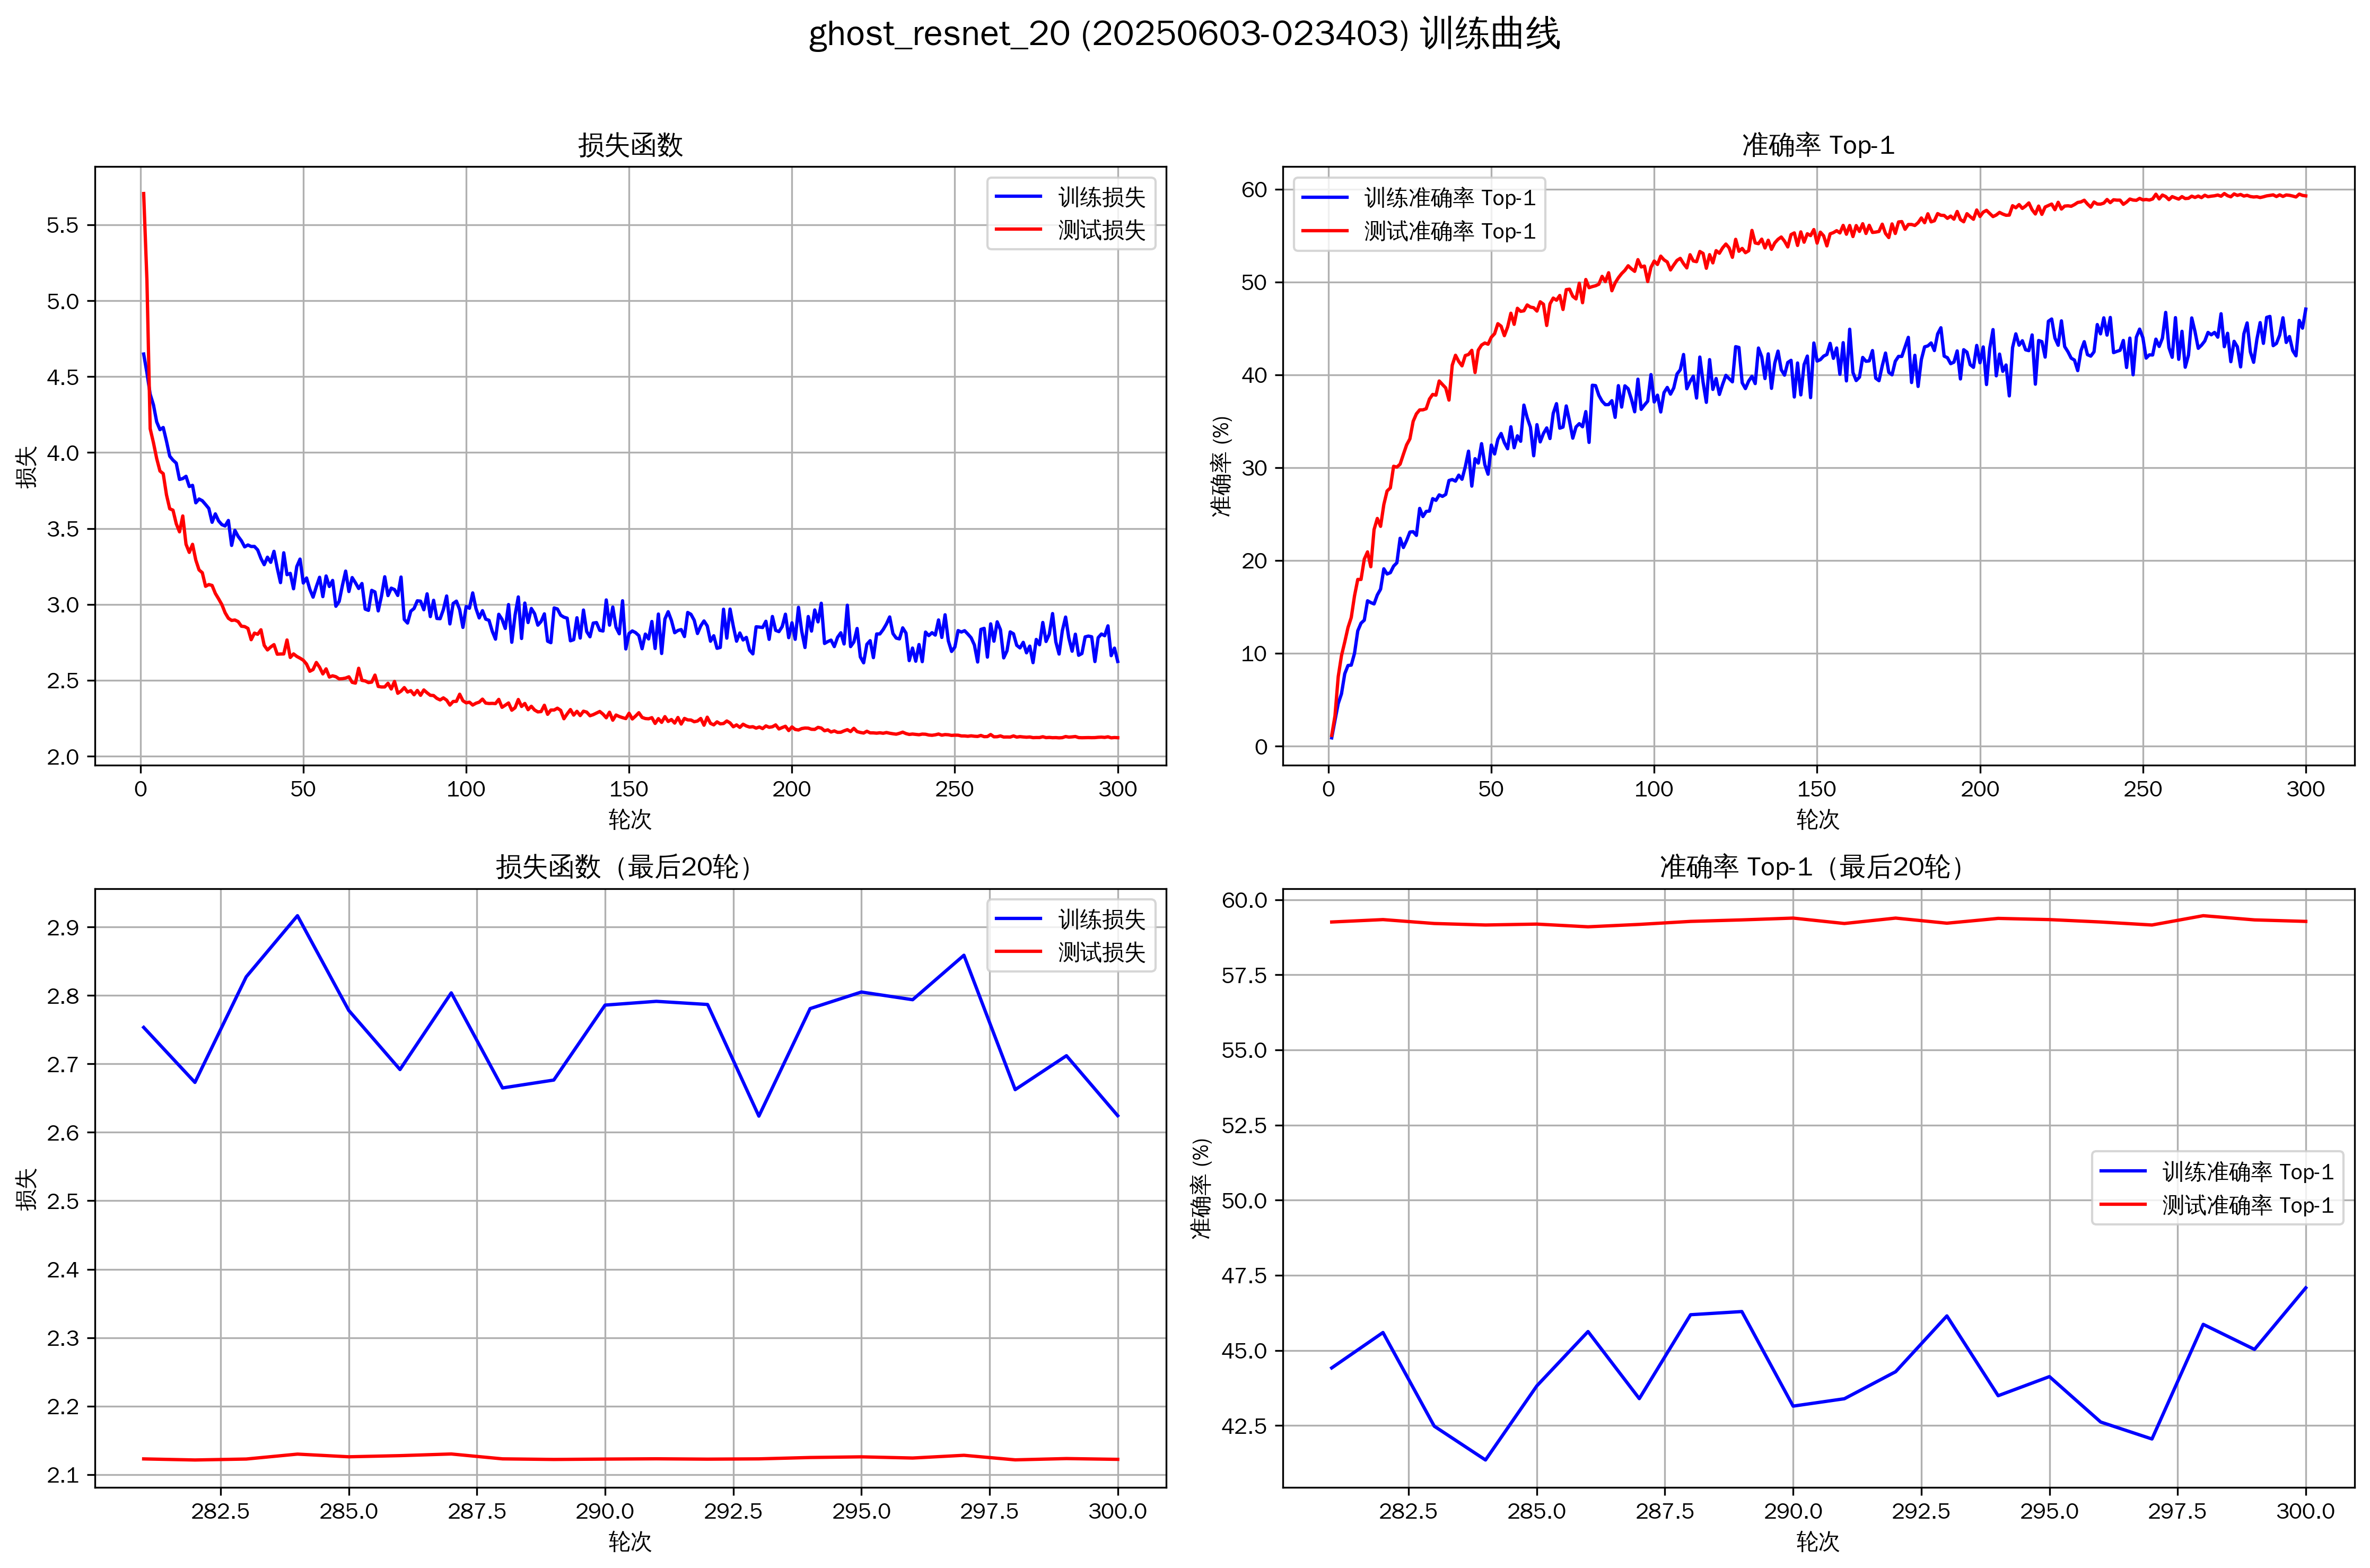
\includegraphics[width=0.9\textwidth]{images/ghost_resnet_20_training_curves.png}
    \caption*{\centering Ghost-ResNet-20: 轻量化模型训练特性}
\end{figure}

\end{frame}

\begin{frame}{\textbf{辅助幻灯片: 补充训练曲线 (3)}}
\frametitle{辅助幻灯片: 补充训练曲线 - ConvNeXt-Tiny}

\begin{figure}[H]
    \centering
    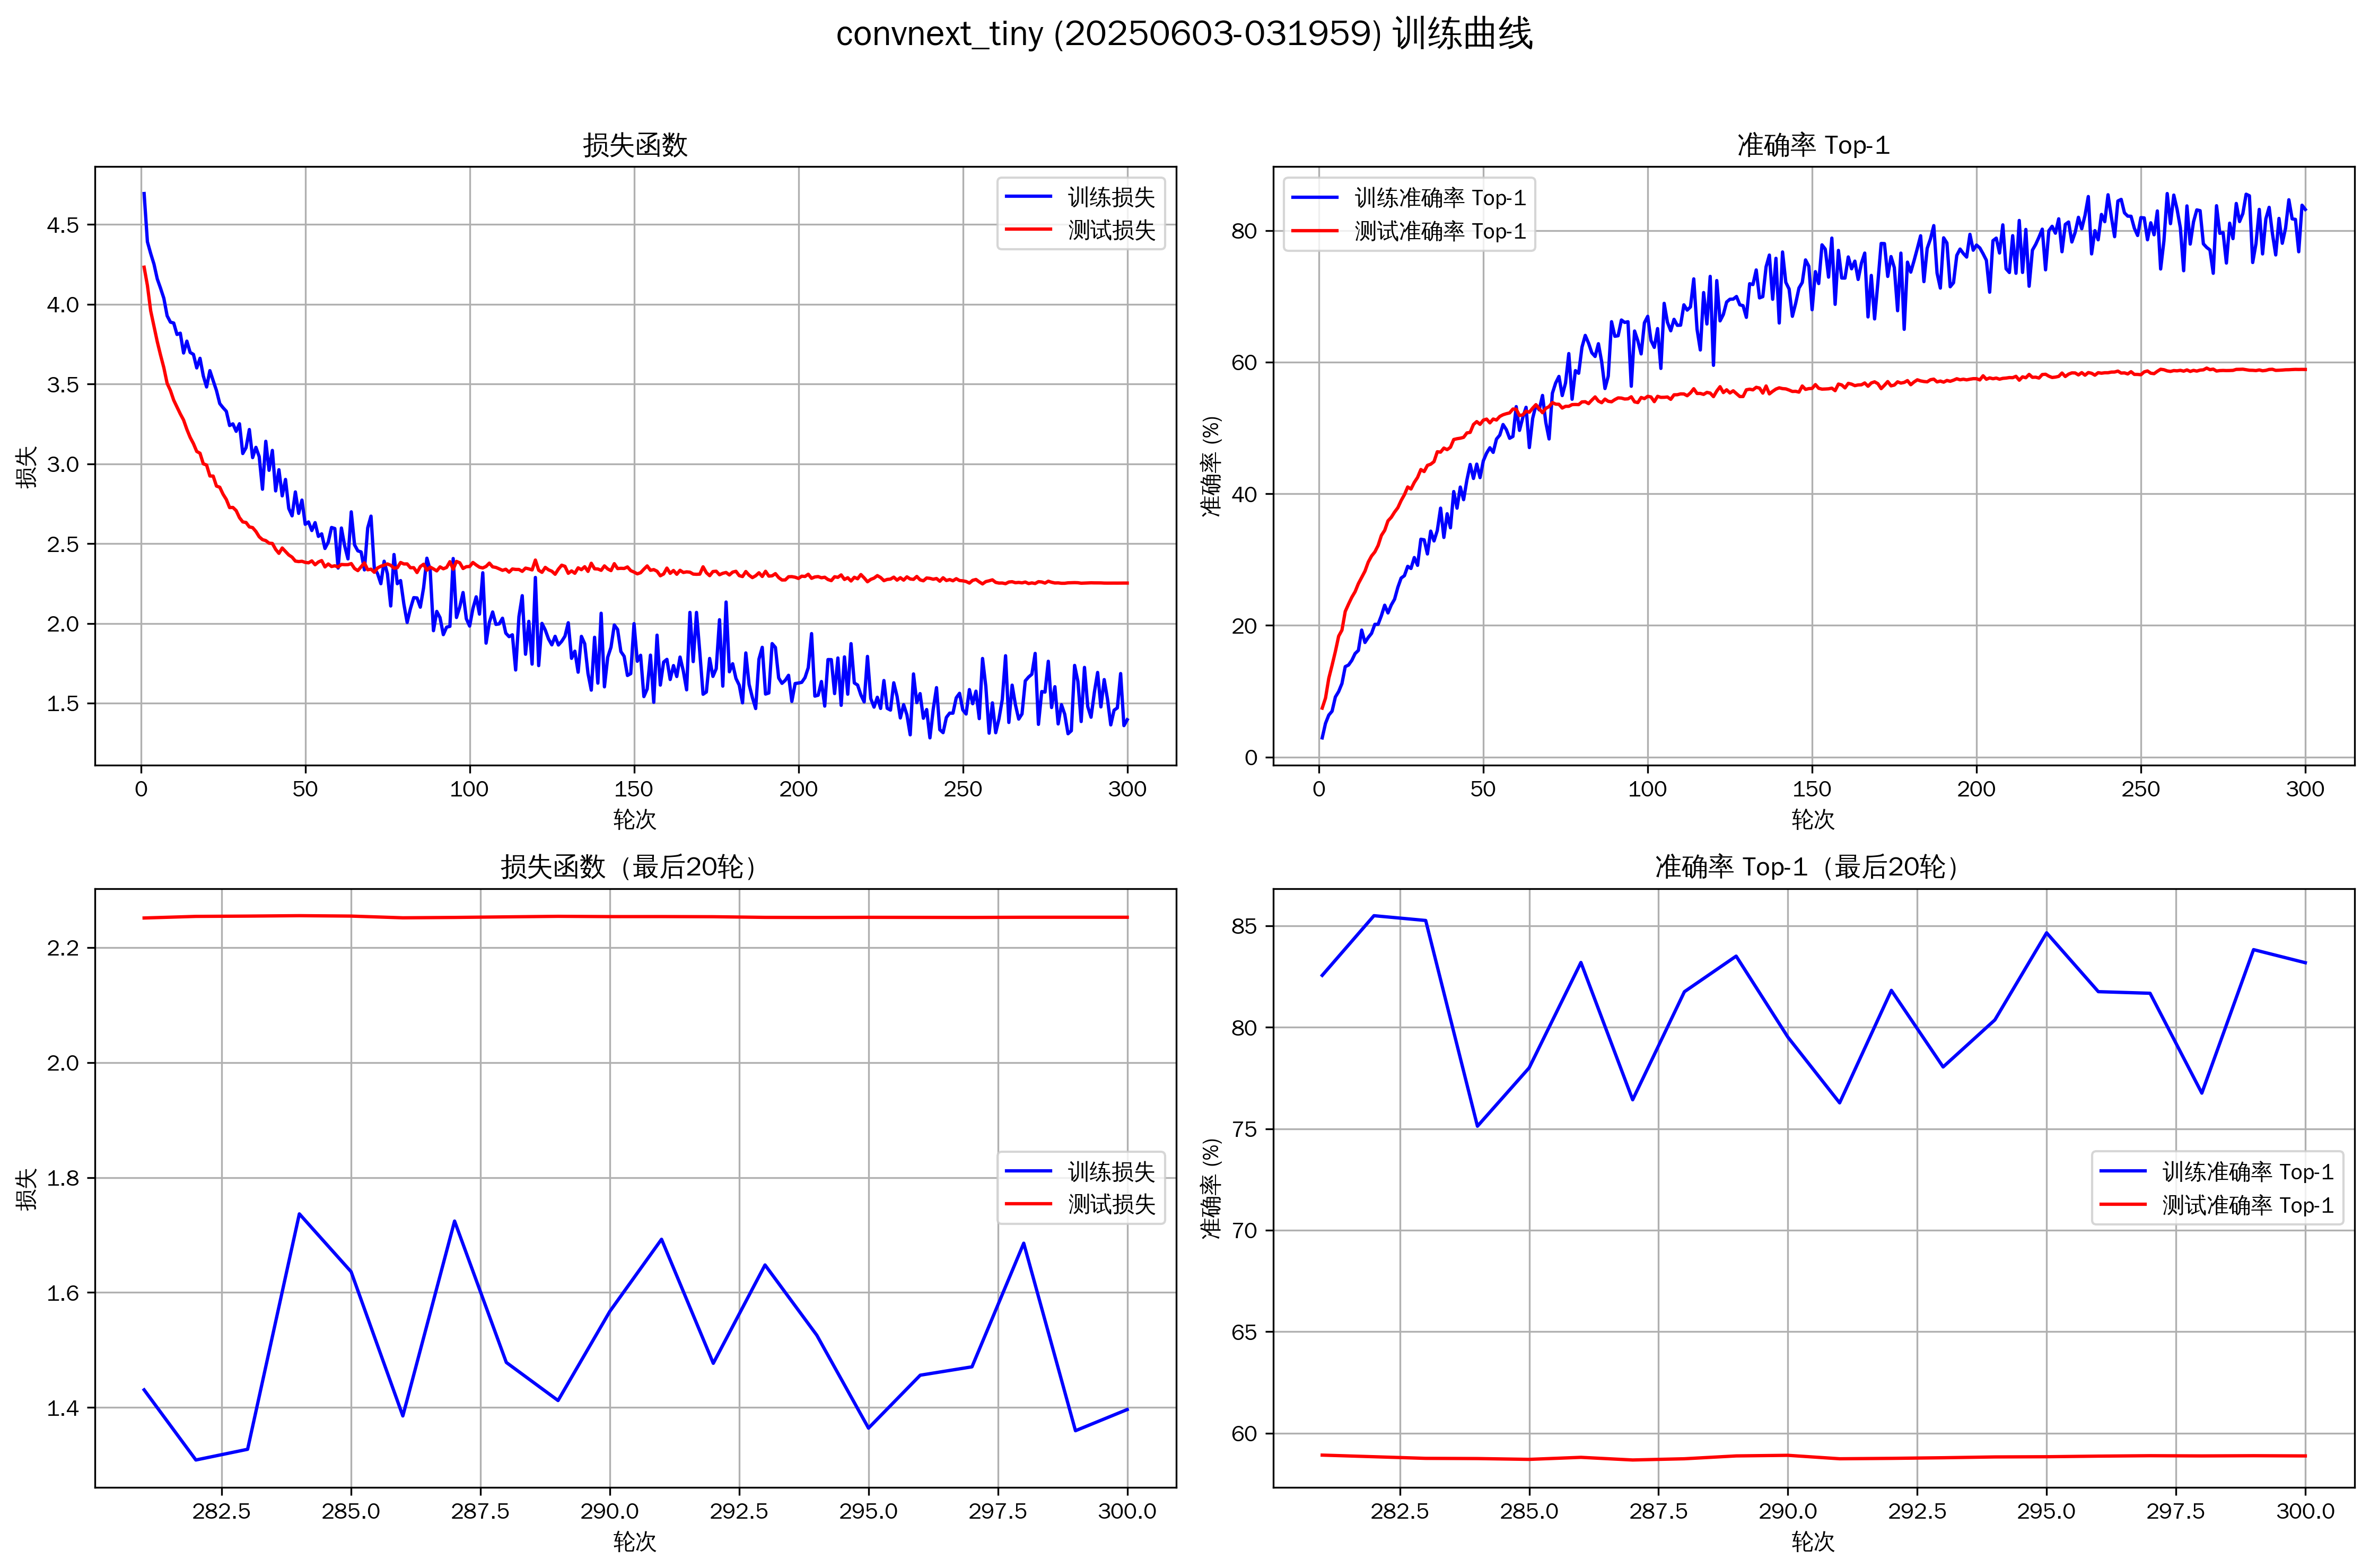
\includegraphics[width=0.9\textwidth]{images/convnext_tiny_training_curves.png}
    \caption*{\centering ConvNeXt-Tiny: 大容量模型过拟合现象}
\end{figure}

\end{frame}

%================================================
%---------------结束页面
%================================================
\setbeamercolor{palette primary}{fg=black, bg=white}
\begin{frame}[standout]
\centering
\Huge{谢谢!}
\vspace{1cm}

\Large{欢迎批评指正}
\end{frame}

%================================================
%---------------参考文献
%================================================
\section*{}
% \appendix
\begin{frame}[allowframebreaks]{参考文献}
\bibliography{bibliografia}
\end{frame}
%================================================
%---------------模板结束
%================================================
\end{document}
